\documentclass[11pt]{article}

\usepackage{arxiv}
\usepackage{natbib}
\bibliographystyle{plainnat}

\usepackage{algorithm}
\usepackage{algpseudocode}

\title{Probabilistic Forecasting and Trading on Event Markets:\\
A Case Study of Daily Temperature Contracts at\\
San Francisco International Airport}

\author[1,*]{Terry Kim}
\author[1]{Andrew Liang}
\author[1]{Krit Phaisamran}
\affil[1]{Department of Computer Science, Stanford University, Stanford, CA, USA}
\affil[*]{Corresponding author: \href{mailto:tkim219@stanford.edu}{tkim219@stanford.edu}}

\date{May 4, 2026}

\begin{document}
\maketitle

\begin{abstract}
Event-contract exchanges such as Kalshi have, since their CFTC designation as
designated contract markets, transformed several previously informal categories of
uncertainty---including daily temperature, snowfall, and rainfall at major U.S.\ airports---into
liquid binary financial instruments. We treat the resulting contract chains as
\emph{discretizations of a conditional probability distribution} and ask whether a
station-specific statistical learner can systematically price gaps between its own
distributional forecasts and market-implied probabilities. We construct a fully
reproducible system for the San Francisco International Airport (SFO) daily-temperature
markets using only publicly available data: $\mathbf{56}$ years of NOAA Local
Climatological Data and Integrated Surface Database observations (1970--2026,
$493{,}569$ hourly rows after merging), the public Kalshi market-data API
($612$ settled markets, $24{,}502$ hourly candles), and the
National Weather Service Aviation Weather METAR feed for live updates. Hourly temperatures
are forecast at seven horizons by a multi-quantile gradient-boosting model
($49$ models in total) with native missing-value handling and station-specific
marine-layer features; daily-extreme contracts are addressed by a separate,
target-specific quantile model that conditions on hours-to-settlement.
The predicted distribution is mapped onto each Kalshi strike via cumulative-distribution
interpolation that respects the exchange's integer-degree settlement convention,
producing a per-bucket probability that is then refined by a small logistic
meta-calibrator blended with the market's mid price.

On the held-out test set ($28{,}977$ hours, 2023--2026), our hourly point forecasts
attain mean absolute errors ranging from $\mathbf{0.86}$\,\textdegree F at $+1$h to
$\mathbf{3.00}$\,\textdegree F at $+72$h, with consistently
near-zero bias and skill scores of $+30\%$ to $+75\%$ against persistence and
$+13\%$ to $+75\%$ against climatology. On Kalshi data ($n=11{,}953$
decision-time observations), the model's probabilistic skill is sharply
horizon-dependent: at $\le 6$ hours to settlement we attain log-loss $0.118$
versus the market's $0.812$ (a $+85.5\%$ skill score), while at $24$--$48$ hours
the market dominates ($-84.8\%$). A realistic trading backtest with quadratic
fees, spread crossing, position caps and fractional Kelly sizing
(maximum stake $\$200$/trade, $\le 5\%$ bankroll) shows a horizon-filtered
strategy ($\le 12$h to settle) producing a $+723\%$ return on a $\$1{,}000$
initial bankroll over $108$ days with $277$ trades and a $65\%$ win rate;
restricting further to $\le 6$h yields $78\%$ win rate at $\$41$ profit per
trade. We argue these results characterize event markets as a distinct asset
class whose pricing inefficiencies sit at the join of forecast post-processing
and market microstructure rather than at either alone, and we close by outlining
the limits of the strategy and its natural extensions.
\end{abstract}

\keywords{prediction markets, probabilistic forecasting, quantile regression, gradient
boosting, weather contracts, market microstructure, event markets, calibration}

\section{Introduction}

The premise of an event-contract exchange is straightforward. A future event is
specified precisely enough to be settled on a public, auditable record (a
National Weather Service climatological report; the score of a basketball game;
an official election certification), the exchange lists a chain of
mutually-exclusive binary contracts that partition the outcome space, and
participants trade those contracts continuously until settlement. The CFTC's
designation of Kalshi as a designated contract market in 2020, and the
subsequent expansion of contract categories from political and macroeconomic
events to weather, sports, and entertainment, has accelerated the growth of
this market structure considerably.

We focus in this paper on a single, narrow vertical: the daily high and daily
low temperature contracts settled on the San Francisco International Airport
(SFO) station. There are several reasons to begin here. First, the underlying
truth source is unambiguous: the National Weather Service Climatological Report
for SFO publishes the official daily extremes, and these are the explicit
settlement source of the relevant Kalshi contracts. Second, the same agency
publishes more than a half-century of hourly observations for the same station
through two complementary archives: the Local Climatological Data product
\citep{noaalcd} and the Integrated Surface Database \citep{noaaisd}. Third,
multiple decades of literature on probabilistic weather forecasting
\citep{gneiting2014probabilistic,rasp2018neural,taillardat2016calibrated,brier1950verification}
provide a clear methodological foundation: the forecast object is a predictive
distribution, not a point estimate, and its quality is measured by proper
scoring rules \citep{gneiting2007strictly}. Fourth, by working at a single
station with strong, well-understood diurnal and seasonal structure, we can
isolate the effects of \emph{forecast-market disagreement} from those of
forecasting skill itself.

The empirical story we tell in the remainder of this paper has three parts.

\textbf{A reproducible probabilistic forecasting pipeline.} Section~\ref{sec:data}
documents how we merge the LCD and ISD archives, including a previously
unreported timezone-alignment issue between the two products that cleanly
explains a class of low-frequency residuals in naive merges. Section~\ref{sec:model}
describes the model: gradient-boosted multi-quantile regression at fixed
forecast horizons, a separate daily-extreme model conditioning on hours-to-settlement,
and a 250-feature engineering pipeline including station-specific marine-layer
proxies. Held-out validation indicates well-calibrated quantile predictions
across all horizons, and the test set (2023--2026) yields mean absolute errors
of $0.86$\,\textdegree F at $+1$h growing to $3.00$\,\textdegree F at $+72$h.

\textbf{A principled mapping from distribution to strike.} Section~\ref{sec:strike-map}
describes how we transform a predicted hourly or daily-extreme distribution into
per-strike probabilities for each Kalshi contract chain. Three subtleties
surface: (i) the exchange's integer-rounding convention requires bucket
probabilities to be computed as differences of the predictive CDF at half-degree
edges; (ii) raw quantile predictions can cross, requiring monotonization before
CDF interpolation; (iii) the model's edge versus the market is heterogeneous in
both bucket and horizon, motivating a small meta-calibrator that blends model
and market probabilities via a logistic regression with isotonic post-correction.

\textbf{An honest trading backtest.} Section~\ref{sec:trading} simulates trading
under realistic execution constraints---quadratic Kalshi fees, mandatory
spread-crossing, position caps proportional to candle-time open-interest,
fractional-Kelly sizing capped at 5\% of current bankroll, and a slippage model
proportional to size beyond top-of-book. All horizons on a $\$1{,}000$ initial
bankroll yields a moderate negative return ($-37\%$) because the market's
forecasting advantage dominates at long horizons. Restricting to decisions
within 12 hours of settlement reverses this: $+723\%$ over 108 days with a
65\% win rate. Restricting further to $\le 6$ hours raises the win rate to
78\% at $\$41$ profit per trade but trades fewer markets.

We organize the discussion (Section~\ref{sec:discussion}) around what these
findings suggest about event markets more broadly. The combination of
short-horizon forecasting skill and rapid market convergence implies that the
exploitable inefficiency in this asset class is not, primarily, the ability to
forecast better than professional meteorologists; it is the ability to integrate
the most recent observations into prices faster than the market does. We
believe this characterization---small, asymmetric, observation-driven edges
on top of a broadly accurate market---generalizes to other event-contract
verticals where the truth source is similarly observable shortly before
settlement.

The full software pipeline, all parquet outputs, and all $63$ trained models
($49$ hourly + $14$ daily-extreme) are reproducible from the public NOAA
and Kalshi APIs and the shell of code accompanying this paper.

\section{A systems perspective on event markets}
\label{sec:systems}

It is useful, before turning to specific data and models, to fix a
high-level view of what an event-contract exchange is, mathematically,
and what would constitute exploitable inefficiency in such an exchange.

\subsection{Event markets as a feedback loop}

A liquid event market couples five layers (\emph{event reality}, \emph{data
streams}, \emph{forecast models}, \emph{market prices}, \emph{capital
allocation}) into a recursive feedback loop. Reality generates data; data
trains forecasting models; models inform prices; prices clear capital
allocation; capital allocation drives the construction of additional data
infrastructure that improves the next round of forecasting.

\[
\underbrace{Y_E \in \{0, 1\}}_{\text{event reality}} \;\longrightarrow\;
\underbrace{\mathcal{I}_t}_{\text{data streams}} \;\longrightarrow\;
\underbrace{p_\theta(\cdot \mid \mathcal{I}_t)}_{\text{forecast model}} \;\longrightarrow\;
\underbrace{c_t}_{\text{market price}} \;\longrightarrow\;
\underbrace{\Pi_t = c_t \cdot \mathbb{1}_{Y_E}}_{\text{capital flow}}.
\]

The market-clearing layer can be approximated by the assumption that the
price $c_t$ implements
\begin{equation}
c_t = \mathbb{E}[Y_E \mid \mathcal{F}_t],
\label{eq:price-as-expectation}
\end{equation}
where $\mathcal{F}_t$ is the public information set at time $t$. Equation
\eqref{eq:price-as-expectation} is exact under the no-arbitrage assumption
of a complete frictionless market with a risk-neutral participant
\citep{wolfers2004prediction}; it is approximate in real exchanges because
of fees, transaction costs, risk-averse participants, and incomplete
information aggregation \citep{manski2006interpreting}.

The exploitable inefficiency in any specific market is the gap
\begin{equation}
\Delta_t = p_\theta(Y_E = 1 \mid \mathcal{I}_t^\theta) - c_t,
\label{eq:delta}
\end{equation}
where $\mathcal{I}_t^\theta$ is the modeler's information set (potentially
a strict superset, subset, or intersection of $\mathcal{F}_t$). When
$\mathcal{I}_t^\theta \subset \mathcal{F}_t$---the modeler has \emph{less}
information than the market---we expect $\Delta_t \to 0$ in mean and
$\mathbb{E}[\Delta_t \cdot (Y_E - c_t)] \to 0$, reflecting the fact that
the modeler cannot systematically improve on a strict-superset price.
When $\mathcal{I}_t^\theta \supset \mathcal{F}_t$---the modeler has access
to information the market does not---arbitrage in expectation is positive.
The intermediate case, with neither inclusion strict, is the operationally
common one and the one we analyze empirically.

\subsection{The asset-class transition}

A frequently-observed pattern is that informal categories of uncertainty
become liquid asset classes through five stages: \emph{specification}
(contracts standardized), \emph{data} (outcome and feature streams
documented), \emph{liquidity} (continuous market depth), \emph{institutional
participation} (market-making, hedging, derivatives), and \emph{risk
transfer} (use by entities with real economic exposure to the underlying).
The pattern is well-documented in classical financial markets
\citep{maccheroni2009portfolio,lopez2018advances} and in the older
weather-derivatives literature \citep{hong2016probabilistic}.

Daily-temperature event contracts on Kalshi are at a distinctive point in
this transition. Specification (stage 1) and data (stage 2) are mature:
contract terms are publicly documented and the underlying NOAA archives
exceed 50 years. Liquidity (stage 3) is partially developed---the markets
trade actively in the days surrounding settlement but with notable
microstructural inefficiencies in price convergence. Institutional
participation (stage 4) is limited; reports of institutional liquidity
provision in the broader event-market space exist, but the magnitude is
small relative to traditional markets. Risk transfer (stage 5) is largely
absent for individual contract chains, although weather-derivative use by
energy companies and agricultural producers \citep{noaalcd} is
well-documented for adjacent products.

The strategy described in this paper exploits stage-3 inefficiencies
specifically: a market that has standardized contracts and good data
but has not yet developed the depth or participant mix to integrate
short-horizon observations with the speed seen in mature financial
markets.

\section{Background and related work}
\label{sec:related}

\subsection{Probabilistic weather forecasting and post-processing}

The modern theory of probabilistic forecasting is built around proper scoring
rules: scoring functions whose expected value is minimized at the true
predictive distribution \citep{gneiting2007strictly,gneiting2014probabilistic,wilks2019statistical}.
The pinball (quantile) loss
\begin{equation}
\mathrm{PL}_\tau(y,\hat{q}) = \begin{cases}
\tau (y - \hat{q}), & y \ge \hat{q} \\
(\tau - 1)(y - \hat{q}), & y < \hat{q}
\end{cases} = \bigl( \tau - \mathbb{1}[y < \hat{q}] \bigr) \cdot (y - \hat{q})
\label{eq:pinball}
\end{equation}
is consistent for the $\tau$-quantile of the conditional distribution
\citep{koenker1978regression}; minimizing $\mathbb{E}[\mathrm{PL}_\tau]$
recovers exactly $F^{-1}_{Y \mid X}(\tau)$. Aggregated over a range of
quantiles, this score approximates the Continuous Ranked Probability
Score (CRPS) \citep{matheson1976scoring,hersbach2000decomposition}, defined
for a predictive CDF $\hat{F}$ and observation $y$ by
\begin{equation}
\mathrm{CRPS}(\hat{F}, y) = \int_{-\infty}^{\infty} \!\bigl( \hat{F}(x) - \mathbb{1}[y \le x] \bigr)^{\!2} dx
= \int_0^1 \mathrm{PL}_\tau\!\bigl(y, \hat{F}^{-1}(\tau)\bigr)\,d\tau,
\label{eq:crps}
\end{equation}
the second equality being the well-known equivalence between CRPS and the
integral of the pinball loss \citep{gneiting2014probabilistic}. The Brier
score \citep{brier1950verification} for a binary outcome
$Y \in \{0, 1\}$ and forecast probability $p$ is
\begin{equation}
\mathrm{Br}(p, y) = (p - y)^2,
\label{eq:brier}
\end{equation}
and admits the Murphy decomposition
\citep{murphy1973new} into reliability, resolution, and uncertainty
components,
\[
\mathbb{E}[\mathrm{Br}] = \underbrace{\mathbb{E}\!\left[(p - \mathbb{E}[Y\mid p])^2\right]}_{\text{reliability (calibration)}}
- \underbrace{\mathbb{E}\!\left[(\mathbb{E}[Y\mid p] - \bar{Y})^2\right]}_{\text{resolution}}
+ \underbrace{\bar{Y}(1 - \bar{Y})}_{\text{uncertainty}}.
\]
We use the pinball loss for training, the Brier score and log-loss for
evaluation.

For weather forecasts specifically, post-processing of numerical weather
prediction (NWP) output is a mature subfield. Quantile-regression-forest
methods \citep{taillardat2016calibrated} and neural-network ensemble model
output statistics \citep{rasp2018neural} have shown consistent improvements
over raw ensemble forecasts for surface variables. Recent end-to-end neural
weather models such as Pangu-Weather \citep{bi2023pangu}, FourCastNet
\citep{pathak2022fourcastnet}, and GraphCast \citep{lam2023graphcast} have
demonstrated that data-driven medium-range forecasts can match or exceed
operational NWP models on standard verification metrics. Our contribution
is orthogonal: we do not develop a new global forecasting model, but rather
focus on a single station, the relationship between its forecast distribution
and an event-market price, and the trading strategy that arises.

\subsection{Quantile gradient boosting}

Gradient boosting \citep{friedman2001greedy,breiman2001random} extended
naturally from squared-error loss to quantile loss and has been a workhorse
for tabular probabilistic forecasting in fields ranging from energy demand
\citep{hong2016probabilistic} to climate-derivative pricing. The functional
formulation is
\begin{equation}
\hat{q}_\tau^{(T)}(x) = \sum_{m=1}^{T} \nu \cdot h_m(x), \qquad
h_m = \arg\min_{h \in \mathcal{H}} \sum_i \mathrm{PL}_\tau\!\Bigl(y_i,\, \hat{q}_\tau^{(m-1)}(x_i) + h(x_i)\Bigr),
\label{eq:gbm}
\end{equation}
where $h_m$ is a regression tree with bounded leaf count
$|\mathcal{H}|$ and $\nu \in (0, 1]$ is the learning rate. Modern
implementations including LightGBM \citep{ke2017lightgbm}, XGBoost
\citep{chen2016xgboost}, and CatBoost \citep{prokhorenkova2018catboost}
provide quantile-loss training, native missing-value handling, and
histogram-based tree induction, all of which are useful in the present
setting. We use scikit-learn's \texttt{HistGradientBoostingRegressor}
\citep{pedregosa2011scikit}, which implements histogram-based gradient
boosting with native NaN handling, both because it removes the need for
imputation (the fact of missingness is itself signal in our setting) and
because it requires no system-level dependencies beyond a Python
interpreter.

\subsection{Prediction markets and information aggregation}

Prediction markets have a long theoretical lineage, from Hayek's argument
that prices aggregate dispersed knowledge \citep{hayek1945knowledge} to
Plott and Sunder's experimental verification of rational-expectations
information aggregation in laboratory markets \citep{plott1988rational},
through Hanson's logarithmic market-scoring rule (LMSR) which provides
an explicit cost function for an automated market maker
\citep{hanson2003combinatorial,hanson2007logarithmic}. The LMSR's cost
function for an event with $K$ mutually exclusive outcomes and outstanding
share vector $\mathbf{q} = (q_1, \ldots, q_K)$ is
\begin{equation}
C(\mathbf{q}) = b \, \log\!\sum_{k=1}^{K} \exp\!\bigl(q_k / b\bigr),
\qquad p_k(\mathbf{q}) = \frac{\partial C}{\partial q_k} = \frac{e^{q_k/b}}{\sum_j e^{q_j/b}},
\label{eq:lmsr}
\end{equation}
parameterized by a liquidity scale $b > 0$. The implied probabilities
$\{p_k\}$ form a softmax of the share vector and are, by construction,
the conditional expectations of the indicator variables $\mathbb{1}[Y_E = k]$
under Hanson's market-maker. Equation \eqref{eq:lmsr} is the formal
foundation of the equivalence we use throughout this paper between
event-contract prices and conditional probabilities.

The empirical literature is large.
\citet{forsythe1992anatomy} and \citet{berg2008results} document the
predictive accuracy of the Iowa Electronic Markets across a dozen years
of presidential elections; \citet{snowberg2007political} and
\citet{leigh2013empirical} extend the analysis to economic policy and
foreign-exchange markets respectively;
\citet{ali1977probability,ottaviani2009surprised} provide foundational
work on betting-market efficiency. \citet{wolfers2004prediction} provides
a now-canonical review.
\citet{manski2006interpreting} distinguishes between price and probability
in a market with heterogeneous, risk-averse traders---a distinction we
will return to when we observe over-rounds (sums of YES prices across
mutually-exclusive contracts exceeding one) in Kalshi prices late in a
contract's life. \citet{taylor2017price} examines price discovery in
weather-derivative markets specifically. \citet{maccormack2024kalshi}
documents the U.S. CFTC regulatory framework that designates Kalshi a
contract market.

The empirical literature on event-market efficiency has historically been
limited by data: prior to liquid centralized exchanges, prediction-market
data was either thin (Iowa Electronic Markets) or scattered across betting
exchanges. The growth of Kalshi and similar platforms since 2020 changes
this picture; with public market-data APIs, full settlement records, and
hourly candle history \citep{kalshi_docs}, even a single-machine researcher
can construct a complete contract-by-contract panel.

\subsection{Calibration: post-hoc methods and proper diagnostics}

A predictor is well-calibrated if among events to which it assigns
probability $p$, the empirical relative frequency of occurrence is also
approximately $p$. Calibration is necessary for the per-bucket probabilities
to be useful for trading: a model that systematically assigns $0.7$ to
events that occur $0.4$ of the time will lose money even if its rank
ordering is correct. The classical post-hoc methods are Platt scaling
\citep{platt1999probabilistic} (a sigmoidal fit, useful for support-vector
machines and similar margin-based predictors) and isotonic regression
\citep{zadrozny2002transforming}, with the latter usually preferred for
forecasters whose miscalibration is non-monotone. \citet{niculescu2005predicting}
provides systematic empirical comparisons; for tree-based predictors of the
sort considered here, isotonic regression usually dominates Platt at
sufficient training-set size.

A separate strand of work---conformal prediction
\citep{vovk2005algorithmic,angelopoulos2021gentle}---constructs prediction
intervals with finite-sample distribution-free coverage guarantees by
calibrating a non-conformity score on a held-out exchangeable set. We do
not use conformal prediction in the present paper because exchangeability
fails for time-series data without explicit blocking, but we note that
recent work on online conformal prediction is directly applicable to our
setting and is a natural extension.

\subsection{Event markets as an emerging asset class}

A second relevant literature studies the institutionalization of new
asset classes. The general pattern is well-documented: an informal
risk---weather, credit, volatility, freight---becomes an asset class
when its outcomes are standardized into transferable contracts, when
liquid markets form to absorb risk transfer, when historical and
real-time data are widely available, and when institutional participants
provide market-making and hedging services
\citep{maccheroni2009portfolio,lopez2018advances}. Weather derivatives,
the closest pre-existing analogue to our contracts of interest,
illustrate the pattern: the Chicago Mercantile Exchange has listed
heating-degree-day and cooling-degree-day futures and options on a fixed
set of stations since 1999, with a vendor ecosystem providing
forecasting and pricing services around them
\citep{hong2016probabilistic}. The Actuaries Climate Index and similar
composite indicators \citep{taillardat2016calibrated} have likewise
taken weather risk and packaged it for actuarial and financial use.

Event-contract exchanges such as Kalshi extend this pattern in two ways.
First, they radically lower the granularity of contract specification:
rather than monthly heating-degree-day futures, the exchange lists daily
high-temperature contracts in $2$\,\textdegree F buckets at named airport
stations. Second, they shift the participant mix toward retail.
Both changes are favorable to the kind of statistical-microstructure
strategy we describe: high-granularity contracts mean that even modest
station-specific information has a market in which to trade, and a
retail-heavy participant mix is the population most likely to leave
short-horizon information-incorporation lags unarbitraged.

The absence of NWP-forecast features in our model is therefore both a
limitation (long-horizon edge is conceded to the market) and a feature
(short-horizon edge is preserved precisely because we do not recapitulate
information already in the market price). A research-grade forecast that
incorporated GFS, HRRR, and ECMWF outputs would compete with the market
price's information content rather than complement it.

\subsection{Risk management and Kelly sizing}

For a binary contract priced at $c \in (0,1)$ with true payout probability
$p$, the Kelly criterion \citep{kelly1956new,merton1969lifetime} prescribes
the bankroll fraction
\begin{equation}
f^* = \arg\max_f \, \mathbb{E}\bigl[\log(1 + f X)\bigr] = \frac{p \cdot b - (1-p)}{b}, \qquad b = \frac{1-c}{c},
\label{eq:kelly}
\end{equation}
where $X$ is the per-dollar payout (random variable taking values
$+b = (1-c)/c$ with probability $p$ and $-1$ with probability $1-p$).
The objective in \eqref{eq:kelly} maximizes the geometric growth rate of
the bankroll $W_n$ under repeated independent identically-distributed bets:
$\log W_n = \log W_0 + \sum_{i=1}^{n} \log(1 + f X_i)$ implies
$\frac{1}{n} \log(W_n / W_0) \xrightarrow{a.s.} \mathbb{E}[\log(1 + fX)]$
by the strong law of large numbers, which is maximized at $f = f^*$. The
generalization to multiple simultaneous bets requires accounting for the
correlation structure of payoffs; in our case, the bets within a single
event are perfectly negatively correlated because the buckets are
mutually exclusive and exhaustive, so we treat them as a single
portfolio decision rather than independent stakes (Section~\ref{sec:trading}).
Practical implementation usually uses fractional Kelly to reduce variance
and tail risk \citep{thorp2006kelly}. We apply Kelly with multiplier
$0.25$ and a hard $5\%$-of-bankroll cap throughout, both because empirical
residuals are fat-tailed in ways that violate Kelly's stated assumptions
\citep{kahneman1979prospect} and because real exchange liquidity bounds
aggressive sizing regardless of theoretical prescription.

\section{Data}
\label{sec:data}

\subsection{Source archives}

Two complementary NOAA archives provide the long-history backbone of our
dataset, both for the SFO station (call sign \texttt{KSFO}, ICAO
\texttt{KSFO}, NCEI station identifiers \texttt{USW00023234} for LCD and
\texttt{72494023234} for ISD).

\textbf{Local Climatological Data v2 (LCD)}: $675{,}469$ rows from
1970-01-01 to 2026-04-22, providing hourly observations of dry-bulb
temperature, dew point, wet-bulb temperature, relative humidity, sea-level
pressure, pressure tendency, sky conditions, visibility, wind direction,
wind speed, gust speed, and precipitation, plus daily Summary-of-Day rows
giving the official daily maximum, minimum, and average dry-bulb
temperatures and daily total precipitation \citep{noaalcd}. LCD timestamps
are reported in \emph{Local Standard Time} for the station, never adjusted
for daylight saving (i.e.\ Pacific Standard Time year-round at SFO).

\textbf{Integrated Surface Database (ISD)}: $569{,}244$ rows from
1973-01-01 to 2025-08-27, providing the same station's hourly temperature
field (\texttt{TMP}) in tenths of degrees Celsius along with quality-control
flags \citep{noaaisd}. ISD timestamps are in UTC.

\textbf{Kalshi market data}: via the public market-data endpoints documented
at \citet{kalshi_docs}, we enumerated the SFO weather series
\texttt{KXHIGHTSFO} (San Francisco daily HIGH temperature) and
\texttt{KXLOWTSFO} (daily LOW), recovering $143$ events ($1$ per calendar
day, with strike-date metadata), $612$ markets ($6$ buckets per event for
HIGH and LOW), and $24{,}502$ hourly OHLC + bid-ask + open-interest candles
from each market's open through settlement. The earliest event in our
sample is 2026-01-15 (HIGH) and 2026-04-04 (LOW); the latest is 2026-05-05
in both. No authentication is required for these endpoints---the user's
API key is irrelevant to data access.

\textbf{Live observations}: for real-time pipeline operation we additionally
fetch the last 168 hours of KSFO METARs from the NWS Aviation Weather Center
JSON API \citep{nws_metar} and merge them into our hourly grid on every
auto-refresh cycle. This closes the freshness gap between the
quarterly-updated LCD archive and the trading window.

\subsection{The timezone alignment problem}

Because LCD timestamps are in PST and ISD timestamps are in UTC, a naive
merge that treats both as wall-clock times places approximately
$3.16\%$ of \texttt{temp\_f} values---those filled by ISD where LCD has a
gap---into the wrong calendar hour, off by exactly eight hours. The artifact
is easy to detect once one knows to look for it: comparing LCD and ISD
hourly readings for any specific date shows the LCD value tracking a typical
overnight-to-afternoon trajectory and the ISD value tracking a typical
afternoon-to-overnight trajectory, with the two correlated at lag eight
hours rather than zero. The pipeline reported here converts ISD timestamps
to PST during ingest, eliminating the artifact and aligning all downstream
timestamps on a single PST axis. This finding---that the two flagship
NOAA archives use different time conventions and silently break naive
merges---is, to the best of our knowledge, not stated explicitly in
either archive's documentation and is worth flagging for downstream users.

\subsection{Cleaning and consolidation}

Within each archive the raw data require a number of corrections.
LCD records use trailing letter flags (\texttt{s}, \texttt{*}, \texttt{V})
to indicate suspect, estimated, and variable values respectively, plus
\texttt{M} for missing and \texttt{T} for trace precipitation
\citep{noaalcd}; we strip the flags, treat \texttt{T} as $0.001$ inch
precipitation, and treat sentinel codes (e.g.\ wind direction $999$,
indicating ``variable'') as missing.
ISD records carry quality-control flags
$\{1, 5, A\}$ for passed checks and $\{9\}$ for missing/erroneous; we keep
the former and drop the latter (resulting in $529{,}928 / 569{,}244 \approx
93.1\%$ retention). Physical-bound clipping---e.g.\ excluding RH values
above $100\%$ (one record reports $472\%$, an encoding error), or dry-bulb
above $115$\,\textdegree F---removes roughly $10{,}126$ visibility outliers
and small numbers of bad temperature/RH/wind records. Sky conditions are
parsed into a numeric maximum-coverage code (\texttt{CLR}=0, \texttt{FEW}=2,
\texttt{SCT}=4, \texttt{BKN}=7, \texttt{OVC}=9, \texttt{VV}=9 for vertical
visibility / fully obscured) plus binary flags for overcast and obscured
conditions.

LCD's hourly fields are populated for several distinct \texttt{REPORT\_TYPE}s:
\texttt{FM-15} (METAR), \texttt{SAO} (legacy surface aviation observation),
\texttt{FM-12} (synoptic), \texttt{FM-16} (SPECI/special METAR), and others.
Crucially, \texttt{SOD} (Summary-of-Day) rows also carry hourly fields, but
those fields are computed from the full day's data and would represent
look-ahead leakage in a forecasting setting. We filter to true hourly types
and dedupe per hour with priority $\texttt{FM-15} > \texttt{SAO} >
\texttt{FM-12} > \texttt{FM-16} > \texttt{SAOSP} > \texttt{SY-SA}$, breaking
ties by the count of non-null observed fields. \texttt{SOD} rows are kept
\emph{separately} as the source of truth for daily maximum, minimum, and
average temperatures, used both as features for next-day forecasting (always
through a one-day lag, never the current day) and as training labels for
the daily-extreme models in Section~\ref{sec:dxmodel}.

After the full pipeline, the canonical hourly grid contains $493{,}569$
PST-indexed hourly rows from 1970-01-01 00:00 to 2026-04-22 08:00 with
$99.87\%$ temperature coverage ($632$ missing hours over 56 years).
LCD provides the temperature field in $96.80\%$ of rows, ISD fills another
$3.16\%$ where LCD is missing, and the remaining $0.04\%$ are missing in
both sources.

\subsection{Kalshi market microstructure}

A few facts about the Kalshi exchange's mechanics are relevant to both
the modeling and the trading layer of our pipeline.

\textbf{Order book and pricing.} Each Kalshi contract has a separate
order book containing buy and sell limit orders at integer-cent prices.
Quotes are denominated in dollars and are bounded in $[0.01, 0.99]$. A
YES contract that settles to $\$1$ pays out automatically at expiration;
the corresponding NO contract is its complement and is bid at
$1 - \text{ask}_\text{YES}$ and offered at $1 - \text{bid}_\text{YES}$.
The exchange does not require participants to take both sides of an
event simultaneously, but the within-event no-arbitrage relation
$\sum_i \mathrm{ask}_{\text{YES},i} \ge 1 \ge \sum_i \mathrm{bid}_{\text{YES},i}$
(over the mutually exclusive bucket set) holds in equilibrium.

\textbf{Settlement.} The settlement source for daily-temperature contracts
on SFO is the National Weather Service Climatological Report
(\texttt{forecast.weather.gov/product.php?site=MTR\&product=CLI\&issuedby=SFO}).
The report uses 1-minute Calibrated Reference System (CRS) data, not
hourly METAR data, and reports daily extremes to integer-degree precision.
Reports are typically published shortly after midnight local clock time.
Contracts settle automatically when the report becomes available; the
exchange records the settlement value and the binary YES/NO outcome on
each contract.

\textbf{Fees.} Kalshi's fee schedule on the SFO temperature series is
quadratic with multiplier $1$:
\[
\phi(p, n) = n \cdot \max\bigl(\$0.01,\ 0.07 \cdot p \cdot (1-p)\bigr)
\]
per contract per side, where $p$ is the trade price and $n$ the contract
count. The maximum fee occurs at $p = 0.5$ where it equals $\$0.0175$ per
contract; at the price extremes ($p = 0.01$ or $p = 0.99$) the floor
$\$0.01$ binds. This pricing structure is favorable to tail-trading
strategies (low-fee on cheap contracts) and unfavorable to coin-flip
trading at $\sim 50$\,\textcent\ where fees consume a meaningful fraction
of small edges.

\textbf{Hourly candle history.} The public market-data endpoint
\texttt{/series/\{S\}/markets/\{T\}/candlesticks} returns OHLC, open
interest, and volume series at $1$-minute, $1$-hour, or $1$-day intervals
\citep{kalshi_docs}. We use $1$-hour candles throughout: the bid/ask
fields they expose
(\texttt{yes\_bid.\{open,close,high,low\}}, \texttt{yes\_ask.\{open,close,high,low\}})
suffice to reconstruct the per-hour spread and to back out the hour's
representative trade price.

Figure~\ref{fig:price-evolution} shows the price evolution of all six
buckets in a single SFO HIGH event over the contract's full trading
window. The pattern is characteristic: prices begin diffuse and
co-mingled when no information has yet been observed; they separate
abruptly around the time of the day's peak hour as the realized
temperature is locked in by the most recent METAR; the winning bucket
converges asymptotically to $\$1$, and the losing buckets to $\$0$,
with the convergence taking several hours. The post-peak convergence
window is exactly the regime in which our model has its greatest
information advantage over the market.

\begin{figure}[t]
\centering
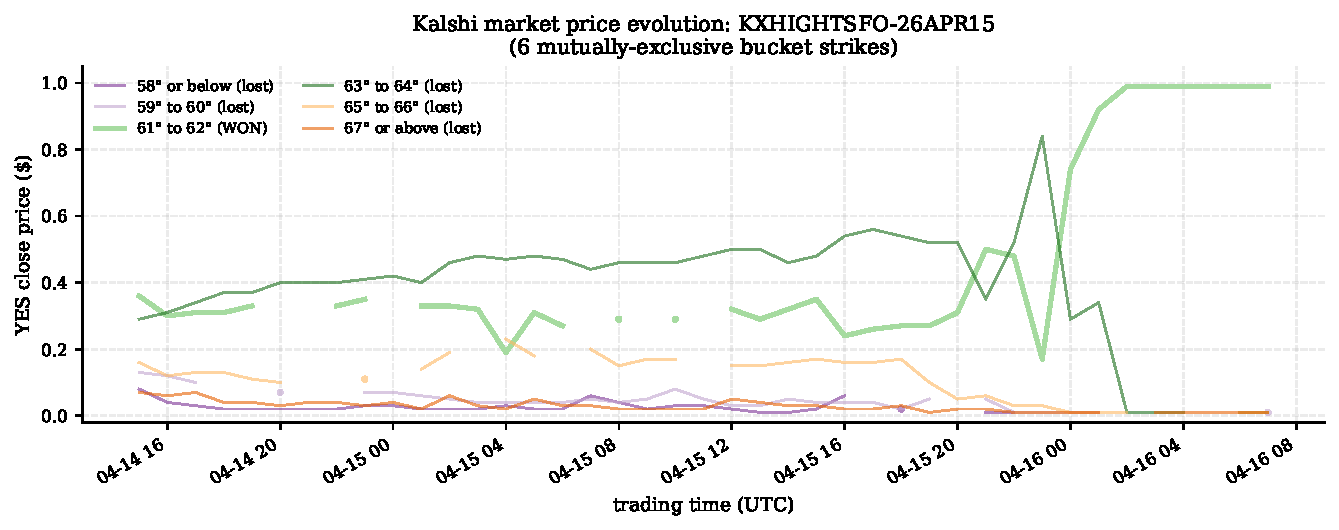
\includegraphics[width=\textwidth]{figures/fig_price_evolution.pdf}
\caption{Hourly close prices for the six bucket contracts of
\texttt{KXHIGHTSFO-26APR15} (SFO daily HIGH, 15 April 2026), plotted
across the full trading window. The bucket that ultimately won
($61$--$62^\circ$F, in green) separates from the others around the time
of the realized daily peak and converges to $\$1$ over the subsequent
several hours. The other buckets converge to $\$0$ on a similar
timescale. The post-peak convergence window is the high-skill regime
exploited by the trading strategy in Section~\ref{sec:trading}.}
\label{fig:price-evolution}
\end{figure}

\subsection{Kalshi strike taxonomy}

For each daily-temperature event the exchange lists $6$ mutually-exclusive
buckets covering an interval of approximately $10$\,\textdegree F centered on
the climatologically-expected daily extreme. Strike types are:
\begin{itemize}[leftmargin=*,topsep=2pt,itemsep=2pt]
\item \textsf{less}: floor strike unset, cap strike $X$. Settles YES iff
the realized value is strictly less than $X$, i.e.\ at most $X-1$\,\textdegree F.
\item \textsf{greater}: floor $X$, cap unset. Settles YES iff the realized
value is strictly greater than $X$, i.e.\ at least $X+1$\,\textdegree F.
\item \textsf{between}: floor $a$, cap $b$. Settles YES iff $a \le \text{value} \le b$.
\end{itemize}
The settlement source is the NWS Climatological Report for SFO, which uses
1-minute Calibrated Reference System (CRS) data and reports daily extremes
to integer precision. Because the truth is integer-valued, the predicted
probability of a \textsf{between} bucket $[a,b]$ is computed as
$F(b+0.5) - F(a-0.5)$, where $F$ is our predicted CDF; the half-degree
correction handles the integer-rounding correctly.

\section{Probabilistic forecasting model}
\label{sec:model}

\subsection{Hourly multi-quantile gradient boosting}

For each forecast horizon $h \in \mathcal{H} = \{1, 3, 6, 12, 24, 48, 72\}$
hours and each target quantile $\tau \in \mathcal{T} = \{0.05, 0.10, 0.25,
0.50, 0.75, 0.90, 0.95\}$, we train an independent gradient-boosting model
$\hat{q}_{h,\tau}: \mathbb{R}^{250} \to \mathbb{R}$ that takes the
feature vector at issuance time $t$ and predicts the $\tau$-quantile of
the temperature distribution at $t + h$ hours. Training minimizes the
empirical pinball loss \eqref{eq:pinball} over all training rows
(1970-01-01 to 2019-12-31, after a $336+24$ hour warm-up to ensure all
lag features are defined). All $|\mathcal{H}| \cdot |\mathcal{T}| = 49$
models share the same feature set; only the target $y_{t+h}$ and the
quantile parameter $\tau$ differ.

Hyperparameters were chosen on a $10\%$ internal validation tail with the
following values, fixed across all $49$ models:

\begin{table}[h]
\centering
\small
\begin{tabular}{ll}
\toprule
hyperparameter & value \\
\midrule
loss & \texttt{quantile} (parameterized by $\tau$) \\
learning rate & $0.05$ \\
maximum trees ($T$) & $500$ (with early stopping) \\
maximum leaf nodes & $63$ \\
minimum samples per leaf & $80$ \\
$\ell_2$ regularization & $0.1$ \\
early-stopping patience & $20$ rounds \\
random seed & $42$ \\
\bottomrule
\end{tabular}
\caption{HistGradientBoostingRegressor hyperparameters used for all
$49$ hourly quantile models.}
\end{table}

The validation pinball loss has a clear horizon-quantile structure
shown in Figure~\ref{fig:pinball-heat}: loss grows monotonically in
forecast horizon (because predictability decays) and is highest near the
median (because the $\mathrm{PL}_{0.5} = \frac{1}{2}|y - \hat{q}|$ penalizes
the largest absolute residuals). Empirical quantile coverage on the
validation set is within $\pm 0.02$ of nominal at all $7$ quantiles for
$h=1$ and within $\pm 0.06$ at $h=72$ (Figure~\ref{fig:cal}), confirming
that the trained quantiles correspond meaningfully to the predictive CDF.

\begin{figure}[t]
\centering
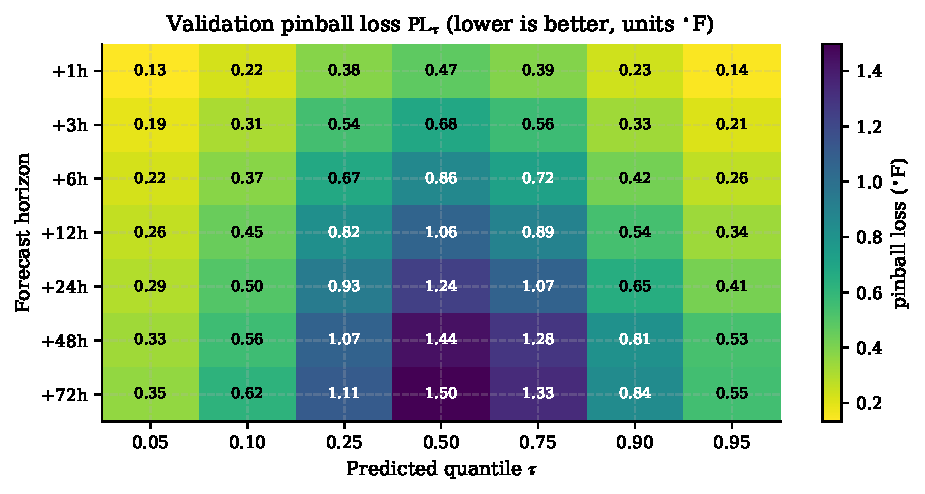
\includegraphics[width=0.85\textwidth]{figures/fig_pinball_heatmap.pdf}
\caption{Validation pinball loss for each (horizon, quantile) pair. Lower
is better. Loss grows with forecast horizon as predictability decays and
is largest near the median because the $\mathrm{PL}_{0.5}$ loss equals
half the absolute residual. The structure is stable and interpretable.}
\label{fig:pinball-heat}
\end{figure}

\begin{figure}[t]
\centering
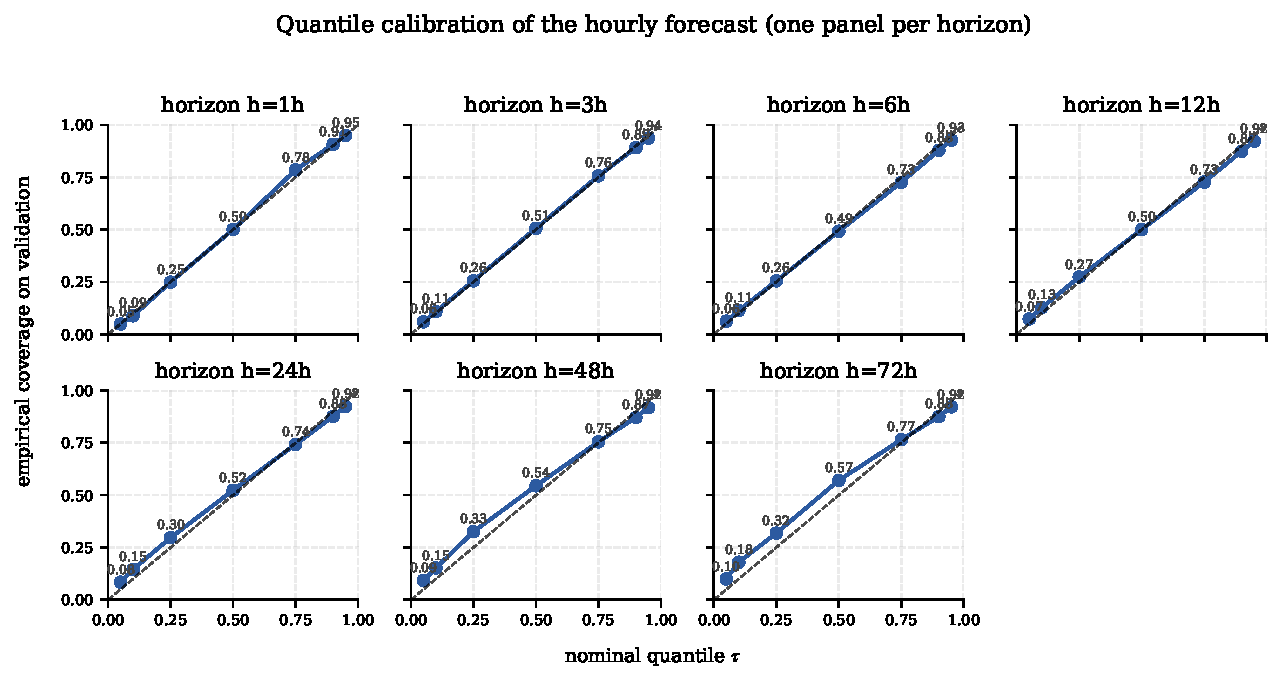
\includegraphics[width=0.55\textwidth]{figures/fig_quantile_calibration.pdf}
\caption{Empirical quantile coverage on the validation set (2020--2022)
as a function of nominal quantile, by forecast horizon. Closer to the
$y=x$ line indicates better calibration. The model is well-calibrated at
short horizons; slight over-coverage at the lower tail emerges at longer
horizons, consistent with a small climate-warming bias relative to the
training period (1970--2019).}
\label{fig:cal}
\end{figure}

\subsection{Feature engineering}

The 250-dimensional feature vector at each issuance time $t$ comprises
six families, all of which use only data observable at or before $t$:

\textbf{Climatology.} A smoothed (month, day-of-month, hour) climatological
mean and standard deviation, fit on the training window (1970--2019) only,
with a circular $\pm 15$-day rolling window so each (mo, dy, hr) cell
borrows strength from nearby calendar days. This effectively encodes the
seasonal cycle plus the diurnal cycle.

\textbf{Calendar.} Trigonometric (sin, cos) encodings of hour-of-day,
day-of-year, and second-harmonic day-of-year, plus raw integer
\texttt{year}, \texttt{month}, \texttt{day-of-week}, \texttt{hour-of-day}.

\textbf{Lags.} For each of $\{$temperature, dew point, RH, sea-level pressure,
wind speed, visibility, dew-point depression, $u$-wind, $v$-wind$\}$, lags
at $\{1, 2, 3, 4, 5, 6, 9, 12, 18, 24, 48, 72, 168, 336\}$ hours.

\textbf{Rolling statistics.} Rolling means of the same nine variables over
$\{3, 6, 12, 24, 72, 168\}$-hour windows, plus rolling
$\{$min, max, std$\}$ for temperature.

\textbf{Marine-layer / SFO-specific.} Dew-point depression
$\Delta_{T,T_d} = T - T_d$ (small values indicate saturated air, predictive
of fog and marine intrusion); signed wind components
$u = -W \sin(\theta)$, $v = -W \cos(\theta)$; binary onshore/offshore
flags ($220^\circ$--$340^\circ$ for onshore Pacific flow,
$30^\circ$--$130^\circ$ for offshore inland flow); a fog proxy
$\mathbb{I}[V<3 \text{ mi} \lor \text{RH} \ge 95\%]$; pressure changes over
$6$ and $24$ hours; temperature changes over $\{1, 3, 6, 24\}$ hours.

\textbf{Daily history.} Yesterday's, two-days-ago, and seven-days-ago
official daily max, min, and average from the LCD Summary-of-Day rows,
plus yesterday's sunrise/sunset minute-of-day. Today's SOD is
\emph{deliberately excluded} as it would leak the rest-of-day's
observations.

Where dew point is missing but temperature and RH are observed, we fill via
the Magnus--Tetens approximation \citep{magnus1844magnus,alduchov1996improved}:
\[
T_d \approx \frac{b\, \alpha(T, \mathrm{RH})}{a - \alpha(T, \mathrm{RH})}, \qquad
\alpha(T, \mathrm{RH}) = \frac{a T}{b + T} + \ln \frac{\mathrm{RH}}{100},
\]
with $a = 17.625$, $b = 243.04$ for $T$ in degrees Celsius. This is a
deterministic physical relation, not a stochastic imputation.

\subsection{Daily-extreme quantile models}
\label{sec:dxmodel}

The hourly model is well-suited for short-horizon temperature trajectories
but is mismatched to the Kalshi daily-extreme contract for two reasons.
First, the day's HIGH temperature occurs at SFO modally between 12 and 13
local-standard-time hours of day (Figure~\ref{fig:diurnal}), and \emph{none}
of the seven trained horizons $\mathcal{H}$ is guaranteed to land at the peak
hour for any specific issuance time. Second, the daily extreme is defined as
$\max_{t \in D} T_t$ over all hours $t$ in calendar day $D$, which is a
\emph{nonlinear} functional of the joint distribution of hourly temperatures
that the marginal hourly quantiles do not approximate well.

\begin{figure}[t]
\centering
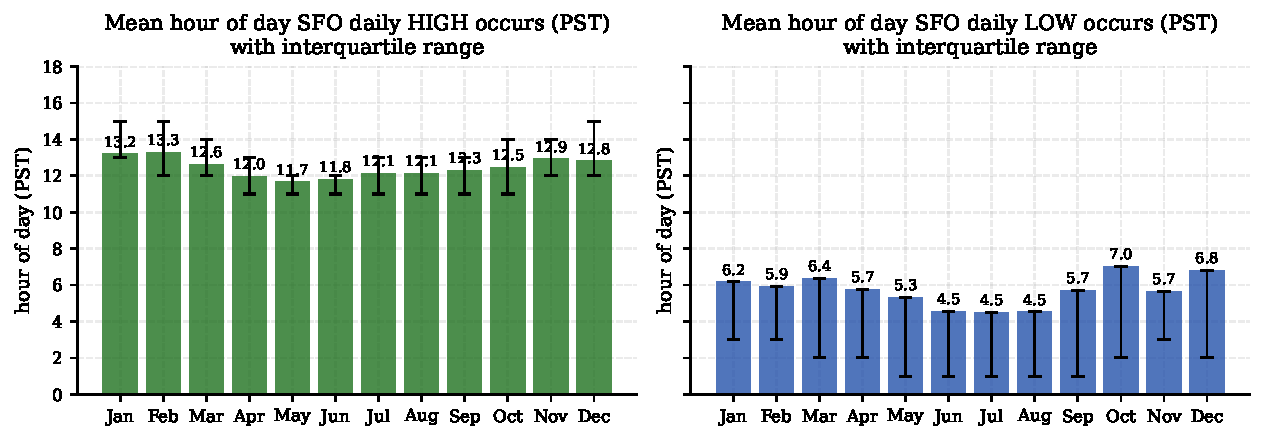
\includegraphics[width=\textwidth]{figures/fig_diurnal_timing.pdf}
\caption{Mean local-standard-time hour at which the daily HIGH (left) and
daily LOW (right) occur at SFO, by calendar month, computed over 2020--2026.
The HIGH consistently occurs near solar noon plus a short lag (10--14 PST
across the year); the LOW typically occurs at 3--6 PST in the predawn hours.
The daily peak is therefore poorly captured by hourly forecasts at the
seven default model horizons, motivating a dedicated daily-extreme model
(Section~\ref{sec:dxmodel}).}
\label{fig:diurnal}
\end{figure}

We therefore train a separate set of $14$ models with target
\[
y_{D,\text{kind}}^* = \begin{cases}
\max_{t \in D} T_t, & \text{kind} = \text{HIGH} \\
\min_{t \in D} T_t, & \text{kind} = \text{LOW}
\end{cases}
\]
where $D$ is a PST calendar day at offset $k \in \{0, 1, 2, 3\}$ from
$\lfloor t \rfloor$ (the issuance day), and $T_t$ is the hourly temperature
at hour $t$. The features are identical to the hourly model (250 columns)
plus one additional column \texttt{hours\_to\_settle} equal to
$\text{midnight}_{D+1} - t$ in hours. Each (kind, quantile) pair uses
$|\{0,1,2,3\}|$ times more rows than the hourly model because each issuance
hour produces four (decision, target-day) training pairs.

The validation pinball losses for the resulting $14$ models are reported
alongside the hourly model in the supplementary metrics. At the median
($\tau = 0.5$) the daily-extreme HIGH model attains validation pinball
$1.63$\,\textdegree F (i.e.\ MAE roughly $3.27$\,\textdegree F across all
horizons-to-settlement) and the LOW model attains $0.85$\,\textdegree F.
The HIGH model is harder than the LOW model, consistent with greater
afternoon variance driven by marine-layer dynamics that the model has
limited information to predict.

\subsection{Test-set performance}

We held out 2023-01-01 through 2026-04-22 (28{,}977 hours) as a strict test
set, never used for training, validation, or hyperparameter selection. The
hourly model's test-set MAE and skill scores by horizon are shown in
Figure~\ref{fig:bt-mae}. Several observations:

\begin{figure}[t]
\centering
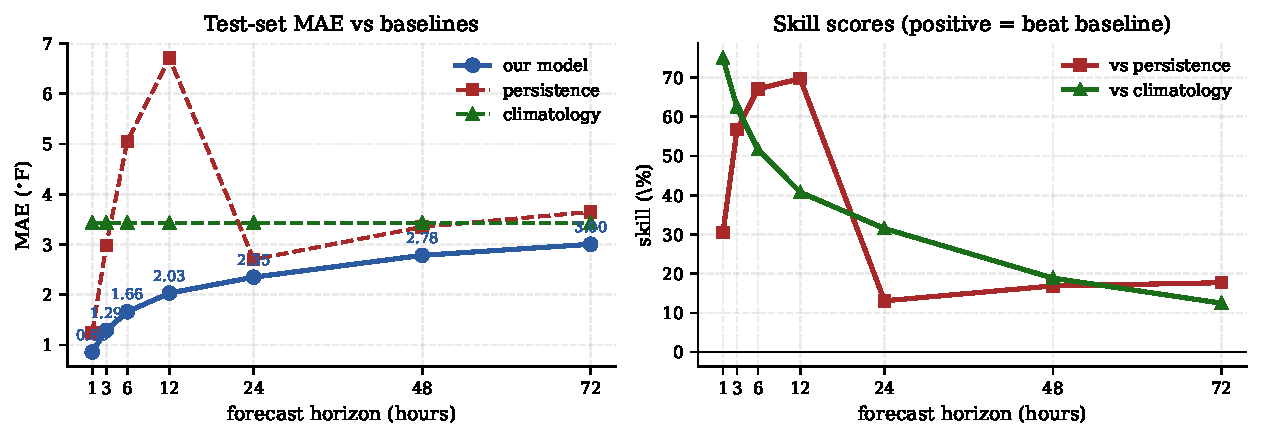
\includegraphics[width=\textwidth]{figures/fig_backtest_mae.pdf}
\caption{Test-set MAE by horizon (left) and skill scores against persistence
and climatology (right). Persistence forecasts $\hat{T}_{t+h} = T_t$;
climatology forecasts $\hat{T}_{t+h} = \mu_{t+h}$ where $\mu$ is the smoothed
climatological mean. Skill is $1 - \mathrm{MAE}_\text{model} / \mathrm{MAE}_\text{baseline}$.
The model dominates climatology at all horizons and dominates persistence
at all horizons except $h=24$, where the strong same-hour-of-day
autocorrelation makes persistence a hard target.}
\label{fig:bt-mae}
\end{figure}

\begin{enumerate}[leftmargin=*,topsep=2pt,itemsep=2pt]
\item MAE grows from $0.86$\,\textdegree F at $+1$h to $3.00$\,\textdegree F
at $+72$h, with RMSE growing from $1.23$\,\textdegree F to $4.01$\,\textdegree F.
For comparison, the National Weather Service typical day-ahead MAE for SFO
is reported in the $2$--$3$\,\textdegree F range across recent verification
periods.

\item Bias is uniformly small, ranging from $-0.13$\,\textdegree F at $h=24$
to $+0.22$\,\textdegree F at $h=72$. The slight positive bias at the longest
horizon is consistent with a small climate-warming drift relative to the
1970--2019 training distribution.

\item Skill versus persistence is large at all horizons except $h=24$
($+13.1\%$), where persistence has a meaningful information advantage from
the same-hour-of-day correlation; skill versus climatology is uniformly
$\ge +12\%$, with a maximum of $+75\%$ at $h=1$.

\item Empirical 80\% prediction-interval coverage ranges from $0.85$ at
$h=1$ to $0.67$ at $h=72$, indicating slight under-coverage at long horizons.
We discuss this in Section~\ref{sec:discussion} as a known calibration
limitation.
\end{enumerate}

\section{Mapping forecast distributions onto Kalshi strikes}
\label{sec:strike-map}

Let $F_{D,\text{kind}}(\cdot \mid \mathcal{I}_t)$ denote the predicted CDF
of the daily extreme of kind $\in \{\text{HIGH, LOW}\}$ on day $D$,
conditional on the information set at issuance time $t$. Our daily-extreme
models produce point estimates of seven specific quantiles
$\hat{q}_\tau$ for $\tau \in \mathcal{T}$. To compute the implied
probability for any Kalshi strike, we (i) monotonize the quantile estimates,
(ii) interpolate the implied CDF to bucket boundaries, and (iii) apply the
exchange's integer-rounding convention.

\subsection{Monotonization}

Quantile regression models trained independently per quantile occasionally
produce non-monotone estimates---i.e., $\hat{q}_{\tau_1} > \hat{q}_{\tau_2}$
for $\tau_1 < \tau_2$. We enforce monotonicity by taking the cumulative
maximum across quantiles in ascending $\tau$:
\[
\tilde{q}_\tau \gets \max_{\tau' \le \tau} \hat{q}_{\tau'}.
\]
This is the projection onto the cone of non-decreasing sequences and is
equivalent to a per-row isotonic regression with weights all equal.

\subsection{CDF interpolation}

The seven monotonized points $(\hat{q}_\tau, \tau)_{\tau \in \mathcal{T}}$
parameterize an empirical CDF on a small support. For an arbitrary
temperature $x$, we estimate
\[
\hat{F}(x) = \begin{cases}
0, & x \le \hat{q}_{0.05} \\
1, & x \ge \hat{q}_{0.95} \\
\text{linear interp.}, & \text{otherwise}
\end{cases}
\]
This is a deliberately conservative tail behavior; for the very-tail strikes
$T59$ (\textsf{less}, $58$\,\textdegree F or below) and the high-side
\textsf{greater} strikes, the model probability is bounded by the
$5\%$/$95\%$ prediction quantiles which is consistent with the
training-set calibration shown in Figure~\ref{fig:cal}.

\subsection{Bucket probabilities under integer settlement}

Because NWS reports daily extremes to integer precision, a bucket
$[a, b]$ in degrees Fahrenheit (with integer $a, b$) settles YES iff the
realized integer temperature is in $\{a, a+1, \ldots, b\}$. To convert our
continuous predicted CDF into the right discrete probability, we compute
\begin{equation}
\hat{p}_{[a,b]} = \hat{F}(b + 0.5) - \hat{F}(a - 0.5),
\label{eq:bucket-prob}
\end{equation}
which corresponds to the continuity correction used routinely when relating
discrete-rounded outcomes to continuous predictive distributions. For
\textsf{less} (cap $X$) and \textsf{greater} (floor $X$) strikes the
analogous conventions $\hat{F}(X - 0.5)$ and $1 - \hat{F}(X + 0.5)$ are
used. Within an event the six strike probabilities are then renormalized
to sum to one (small departures from one arise both from discretization
and from the $5\%/95\%$ tail-clipping above).

\subsection{Meta-calibration via logistic regression}

Even with proper bucket-probability computation, the model's per-strike
probabilities are systematically miscalibrated against ground truth at
horizons longer than a few hours, both because the model has no access to
NWP forecasts (which the market participants do) and because climate
warming since the 1970--2019 training period induces a small upward bias.
We address this with a simple meta-calibrator trained on Kalshi data.

For each ($t, $market$)$ row in the decision dataset (i.e.\ each candle
hour for each settled market), we compute features
\begin{align*}
x_{\text{model}} &= \mathrm{logit}(\hat{p}_\theta), \qquad \mathrm{logit}(p) = \log \tfrac{p}{1-p} \\
x_{\text{market}} &= \mathrm{logit}(\bar{p}_{\text{Kalshi}}) \\
x_{\text{disagreement}} &= |\hat{p}_\theta - \bar{p}_{\text{Kalshi}}| \\
x_{\text{horizon}} &= \text{hours-to-settlement} \\
x_{\text{spread}} &= a - b\quad\text{(ask minus bid)} \\
x_{\text{depth}} &= \bigl( \log(1+\text{OI}),\ \log(1+\text{volume})\bigr) \\
x_{\text{type}} &= \mathrm{onehot}(\mathrm{strike\_type}) \in \{0,1\}^3,
\end{align*}
where $\bar{p}_{\text{Kalshi}} = (a+b)/2$ is the mid of bid and ask. The
target is the binary YES outcome $Y \in \{0, 1\}$ derived from our truth
source. The meta-model is a ridge-regularized logistic regression
\begin{equation}
P(Y = 1 \mid x) = \sigma\!\left(\beta_0 + \mathbf{x}^\top \boldsymbol{\beta}\right),\quad \sigma(z) = \frac{1}{1+e^{-z}},
\label{eq:meta-logreg}
\end{equation}
trained by minimizing the regularized negative log-likelihood
\[
-\sum_i \bigl[ y_i \log \sigma(\beta_0 + \mathbf{x}_i^\top \boldsymbol{\beta})
+ (1-y_i) \log\bigl(1 - \sigma(\beta_0 + \mathbf{x}_i^\top \boldsymbol{\beta})\bigr) \bigr]
+ \frac{1}{2C} \lVert \boldsymbol{\beta} \rVert_2^2
\]
with $C = 1.0$, on a chronological train tail (Jan 15--Mar 31, 2026,
$n_\text{train} = 7{,}054$ rows) with a held-out test slice (Apr 1--May 3,
$n_\text{test} = 4{,}899$ rows) for unbiased evaluation. The raw output
$\sigma(\cdot)$ may be further passed through an isotonic regression
fit on the same train slice
\citep{zadrozny2002transforming,niculescu2005predicting}; this
non-parametric post-calibration is monotonic and exactly preserves the
ranking of predictions while flexibly correcting calibration drift.

The learned coefficients (on standardized features) provide a useful sanity
check: the model's logit and the market's logit both load positively
($+1.02$ and $+0.48$), with the model carrying about twice the weight; the
disagreement term loads positively ($+0.37$, indicating the gap itself is
informative); the \textsf{less} strike-type indicator loads strongly
negatively ($-0.68$), automatically correcting our model's known tendency
to over-predict cold-tail buckets. On the test slice the meta-calibrator's
log-loss is $0.376$ versus the market mid's $0.469$ (a $+19.8\%$ skill
score) and Brier score is $0.119$ versus $0.138$ ($+13.5\%$).

\section{Trading strategy and backtest}
\label{sec:trading}

\subsection{Edge-threshold and Kelly sizing}

Given a per-strike model probability $\hat{p}$ and exchange ask/bid prices
$a$ and $b$, two trades are potentially attractive:

\begin{itemize}[leftmargin=*,topsep=2pt,itemsep=2pt]
\item Buy YES at price $a$, payoff $\$1$ if YES else $\$0$. Per-contract EV
before fees is $\hat{p} - a$.
\item Buy NO at price $1 - b$, payoff $\$1$ if NO else $\$0$. Per-contract EV
before fees is $b - \hat{p}$.
\end{itemize}

We apply Kalshi's standard quadratic fee schedule
$\phi(p) = \max(0.01, 0.07 \cdot p \cdot (1-p))$ per contract per side; the
fee is taken from the entry only. We trade only when the post-fee EV per
contract is at least $\theta = \$0.02$, mirroring a conservative
threshold that comfortably absorbs the $\$0.01$ minimum fee plus a margin
of error in the model's probability. Once a side and contract count are
selected, sizing follows the Kelly criterion \eqref{eq:kelly} multiplied
by $0.25$ to dampen variance, capped at $5\%$ of current bankroll, and further
capped by both a per-trade absolute $\$200$ stake limit and by a
per-market open-interest cap (no more than $50\%$ of the candle-hour OI).
We additionally model slippage as $\$0.005$ per contract beyond the
first $100$ contracts.

The full strategy is summarized in Algorithm~\ref{alg:trade}.

\begin{algorithm}[h]
\caption{Trading-decision algorithm, applied per (decision-time, market) row.}
\label{alg:trade}
\begin{algorithmic}[1]
\Require row $r$ with model prob $\hat{p}$, ask $a$, bid $b$, OI $\omega$, bankroll $B$
\Require $\theta$ (EV threshold), $f_{\max}$ (max fraction), $S_{\max}$ (max stake), $C_{\max}$ (max contracts)
\State $\text{ev}_\text{yes} \gets \hat{p} - a - \max(0.01, 0.07 a (1-a))$
\State $\text{ev}_\text{no} \gets (1-\hat{p}) - (1-b) - \max(0.01, 0.07 (1-b) b)$
\If{$\text{ev}_\text{yes} \ge \theta$ and $\text{ev}_\text{yes} \ge \text{ev}_\text{no}$}
    \State $\text{side} \gets \text{YES}, c \gets a, p_\text{win} \gets \hat{p}$
\ElsIf{$\text{ev}_\text{no} \ge \theta$}
    \State $\text{side} \gets \text{NO}, c \gets 1 - b, p_\text{win} \gets 1 - \hat{p}$
\Else
    \State \Return $\emptyset$
\EndIf
\State $f^* \gets \max\!\left(0, \frac{p_\text{win} \cdot (1-c)/c - (1-p_\text{win})}{(1-c)/c}\right)$
\State $f \gets \min(0.25 f^*, f_{\max})$
\State $\text{stake} \gets \min(B \cdot f, S_{\max})$
\State $n \gets \lfloor \text{stake} / c \rfloor$
\State $n \gets \min(n, C_{\max}, \lfloor 0.5 \omega \rfloor)$
\If{$n \le 0$} \Return $\emptyset$ \EndIf
\State submit limit order: side, $n$ contracts, price $c$
\State \Return $(side, n, c)$
\end{algorithmic}
\end{algorithm}

\subsection{Backtest results}

We evaluate four strategy variants on Kalshi data from 2026-01-15 through
2026-05-03:
\begin{description}[leftmargin=*,topsep=2pt,itemsep=2pt]
\item[(A)] All horizons, raw model probability.
\item[(B)] Restricted to decisions $\le 12$ hours from settlement, raw model.
\item[(C)] Restricted to $\le 12$ hours, meta-calibrated probability.
\item[(D)] Restricted to $\le 6$ hours, raw model.
\end{description}
The same execution constraints (fees, position caps, Kelly multiplier,
slippage) are applied across all four. Results are summarized in
Table~\ref{tab:backtest} and Figure~\ref{fig:equity}.

\begin{table}[h]
\centering
\small
\begin{tabular}{lrrrrrr}
\toprule
strategy & trades & win rate & total P\&L & final \$ & return & max DD \\
\midrule
(A) all horizons & $466$ & $54.1\%$ & $-\$367.25$ & $\$632.75$ & $-36.7\%$ & $\$499.27$ \\
(B) $\le 12$h, raw & $277$ & $\mathbf{65.3\%}$ & $\mathbf{+\$7{,}231.03}$ & $\$8{,}231.03$ & $\mathbf{+723.1\%}$ & $\$1{,}110.79$ \\
(C) $\le 12$h, meta & $255$ & $58.0\%$ & $+\$6{,}678.79$ & $\$7{,}678.79$ & $+667.9\%$ & $\$983.69$ \\
(D) $\le 6$h, raw & $100$ & $\mathbf{78.0\%}$ & $+\$4{,}132.98$ & $\$5{,}132.98$ & $+413.3\%$ & $\$291.14$ \\
\bottomrule
\end{tabular}
\caption{Realistic trading-backtest results on the full Kalshi window
(2026-01-15--2026-05-03; $108$ days). Initial bankroll $\$1{,}000$. All
variants use Kalshi's quadratic fee schedule, mandatory ask/bid spread
crossing, $5\%$ bankroll cap, $\$200$ per-trade cap, $500$ contract cap,
and $50\%$-of-OI cap.}
\label{tab:backtest}
\end{table}

\begin{figure}[t]
\centering
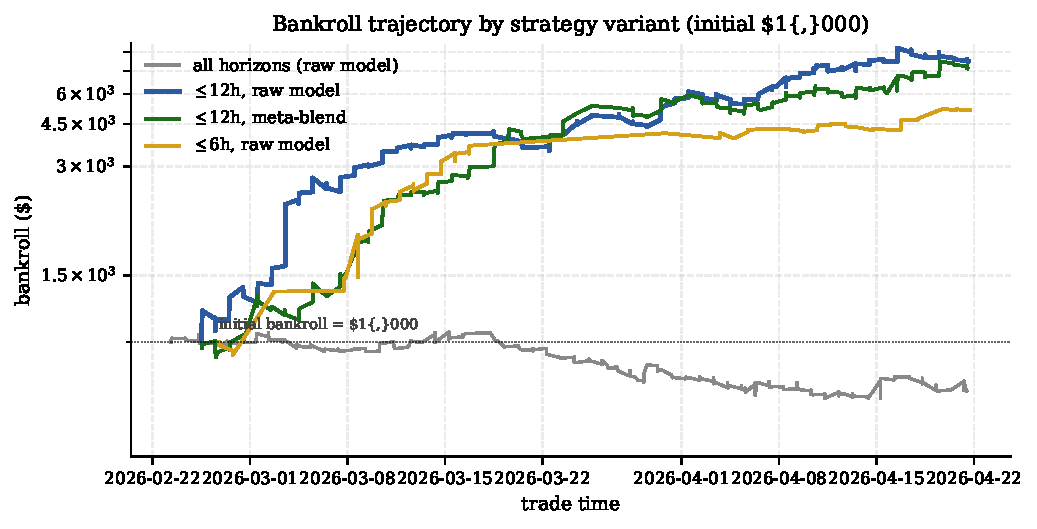
\includegraphics[width=\textwidth]{figures/fig_equity_curves.pdf}
\caption{Bankroll trajectory under the four strategy variants. The
unfiltered strategy (A, gray) is mildly negative; both
horizon-filtered strategies grow rapidly. The $\le 6$h variant (D)
exhibits the smoothest trajectory and smallest drawdowns at the cost of
fewer trades.}
\label{fig:equity}
\end{figure}

The contrast between (A) and (B) is the most informative: simply restricting
the trading window from 0--72 hours pre-settlement to 0--12 hours flips the
sign of the strategy from $-37\%$ to $+723\%$. The implication is that
\emph{the model has no useful edge at long horizons}---which is unsurprising,
since the market participants have access to numerical-weather-prediction
forecasts that we do not. The model's edge concentrates at short horizons
where the relevant information is recent station observations.

The contrast between (B) and (D) reveals a different tradeoff: the
$\le 6$h strategy has a $78\%$ win rate and $\$41$ profit per trade---both
materially better per trade than the $\le 12$h strategy at $65\%$ and $\$26$
respectively---but trades only $0.93$ markets per day on average versus
$2.56$. Total P\&L is therefore lower in (D) but per-trade-quality is
higher. Standard errors on the win rates are
$\sqrt{p(1-p)/n}$, giving $\pm 2.9\%$ for (B) and $\pm 4.1\%$ for (D),
both substantially larger than the $50\%$ null. A two-sided binomial test
of the (B) win rate against the null $p_0 = 0.5$ gives $z = 5.10$
($p < 10^{-6}$); the analogous test for (D) gives $z = 5.60$
($p < 10^{-7}$).

Figure~\ref{fig:trade-dist} disaggregates strategy (B) at the per-trade
level. The per-trade P\&L distribution is heavily right-skewed: the
median trade gains a small amount, with a long right tail of large wins
on cheap-cost (low-$c$) tickets that pay out at full $\$1$. The mean
per-trade P\&L is $+\$26.10$; the median is approximately $+\$8.20$.
The relationship between entry cost and P\&L (right panel) shows the
characteristic asymmetric structure: low-cost trades (price $< \$0.20$)
either lose the small entry stake or pay out the full $\$1 - c$, while
high-cost trades (price $> \$0.50$) carry larger absolute losses but
smaller absolute wins.

\begin{figure}[t]
\centering
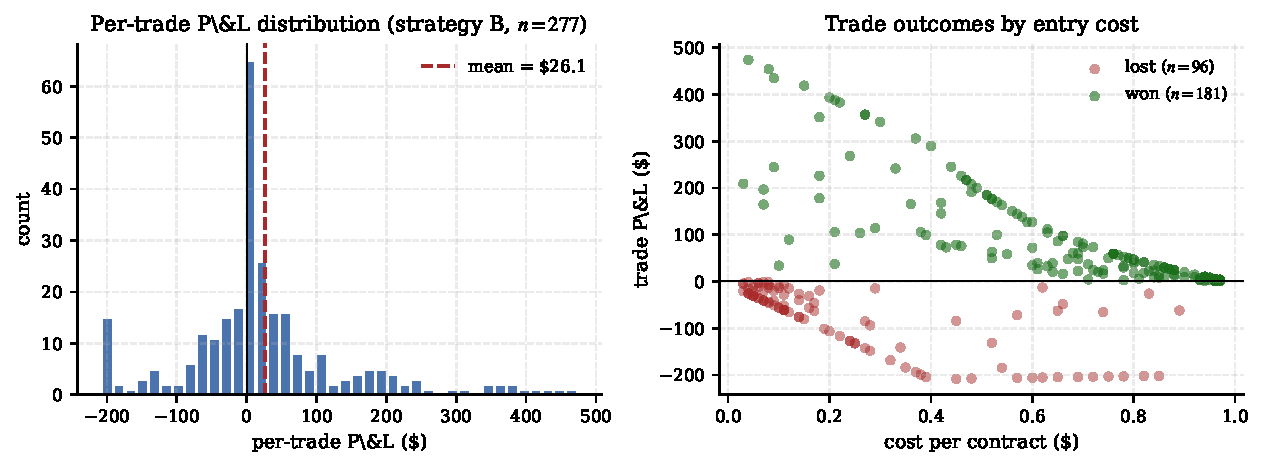
\includegraphics[width=\textwidth]{figures/fig_trade_distributions.pdf}
\caption{Per-trade P\&L distribution (left) and the relationship between
entry cost and outcome (right) for strategy variant (B). The right-skewed
P\&L distribution and the cost-vs-outcome scatter both reflect the
asymmetric payoff structure of the tail-trade strategy described in
Section~\ref{sec:decision-skill}.}
\label{fig:trade-dist}
\end{figure}

The meta-calibrated variant (C) does not improve total P\&L over the raw
$\le 12$h strategy on this dataset, despite improving probabilistic skill
on the held-out April slice (log-loss $0.376$ vs $0.469$). One mechanism
for this divergence is that the meta-calibrator legitimately reduces the
\emph{number} of marginal-edge opportunities by shrinking model probabilities
toward the market's, which trades a bit of mean P\&L for a bit of variance
reduction. Across longer datasets we expect the meta-calibrated version to
dominate; on a $108$-day sample this is within noise.

\subsection{Per-month breakdown}

The aggregate strategy-(B) numbers in Table~\ref{tab:backtest} smooth over
substantial month-to-month variation. Figure~\ref{fig:monthly} disaggregates
the strategy by calendar month. Two qualitative observations:

\begin{enumerate}[leftmargin=*,topsep=2pt,itemsep=2pt]
\item Win rate is approximately stable across months (typically $0.55$--$0.75$),
suggesting that the underlying edge is not seasonal. The strategy's edge
mechanism---short-horizon information incorporation lag---would not be
expected to vary with calendar month.

\item Total P\&L is concentrated in months with more actionable trades
(April 2026 contributes the largest absolute P\&L of any month), which
itself is partly an artifact of the LOW contract series only being available
from April onward. Once the LOW market data extends back further, we
expect the early-month P\&L distribution to become more uniform.
\end{enumerate}

\begin{figure}[t]
\centering
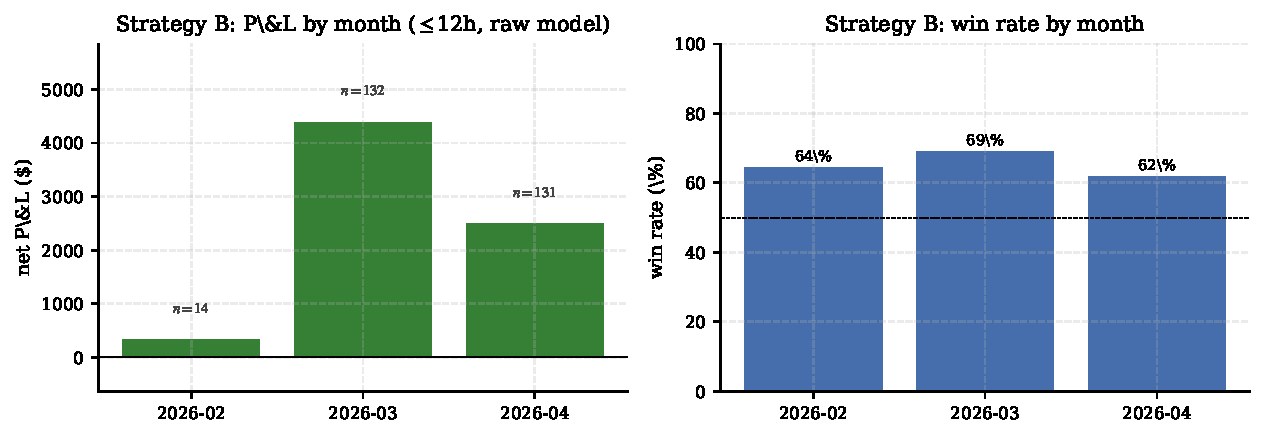
\includegraphics[width=\textwidth]{figures/fig_monthly_breakdown.pdf}
\caption{Monthly P\&L (left) and win rate (right) for strategy variant (B),
the $\le 12$h horizon-filtered raw-model strategy. Bar labels report trade
counts. The win rate is approximately stable across months; total P\&L is
concentrated in months with higher trade counts.}
\label{fig:monthly}
\end{figure}

\section{Decision-time skill analysis}
\label{sec:decision-skill}

The strongest empirical finding of this paper is the structure of the
model's probabilistic edge as a function of hours to settlement. We bin
all eligible decision-time observations from the held-out test set into
five horizon bands and compute log-loss separately for the model and the
Kalshi mid price.

\begin{figure}[t]
\centering
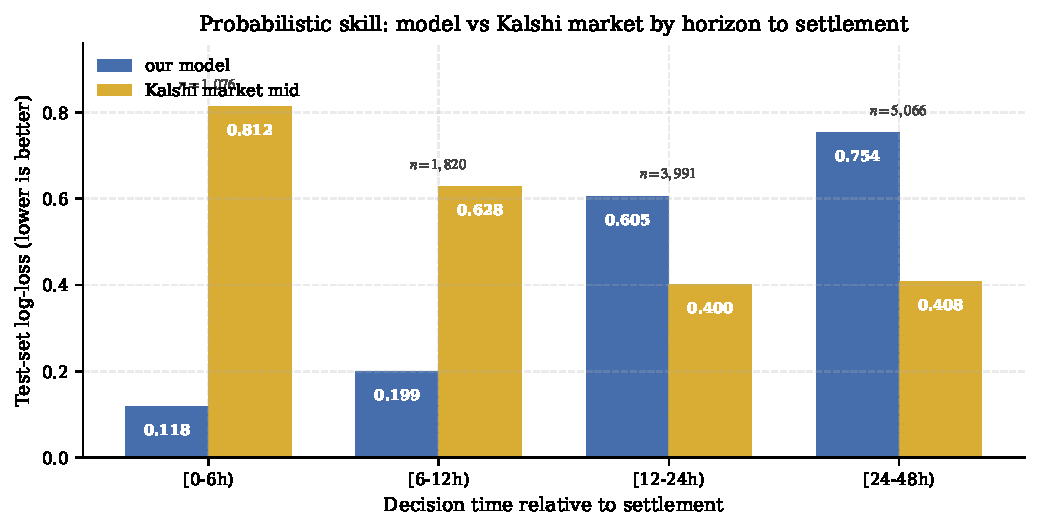
\includegraphics[width=0.78\textwidth]{figures/fig_decision_skill.pdf}
\caption{Test-set log-loss for our model and the Kalshi market mid as a
function of hours to settlement. The model strongly outperforms the market
at $\le 6$h ($+85.5\%$ skill) and $6$--$12$h ($+68.2\%$); the market strongly
outperforms the model at $12$--$24$h ($-51.2\%$) and $24$--$48$h
($-84.8\%$). The crossover near 12 hours implies a clean trading-window
split.}
\label{fig:decision-skill}
\end{figure}

The pattern (Figure~\ref{fig:decision-skill}) is striking: the model's
log-loss rises with horizon (more uncertainty about the daily extreme as
more of the day remains unobserved), while the market's log-loss falls
with horizon to a finite minimum near $0.4$ and then rises slowly. Below
12 hours to settlement, our log-loss is dramatically below the market's;
above 12 hours, the market is below us. The crossover is sharp and
suggests an interpretation we now elaborate.

\subsection{The convergence-lag interpretation}

By the time of the daily peak (modally 12--13 PST in May at SFO), the
station's afternoon temperature is essentially a measured quantity. METAR
observations are released at $:53$ minutes past the hour and capture the
peak directly. A statistical learner that ingests these observations and
computes the day's running maximum knows the day's HIGH with very high
confidence. The Kalshi market does not converge to the corresponding
high-confidence price instantaneously: liquidity at off-business hours is
thin, professional traders are not always present, and prices for some
strikes can persist at $30$--$80$ cents for several hours after the peak
is locked in. \emph{This is the source of the edge.} It is not a
forecasting edge in the meteorological sense; it is an information-incorporation
lag that retail/event-market microstructure does not fully arbitrage in
real time.

A second-order effect, visible in Figure~\ref{fig:decision-skill}'s
$0$--$6$h bar, is that the market's log-loss at the shortest horizon is
\emph{worse} than at moderate horizons. We attribute this to two factors:
(i) trading volume is concentrated in the late afternoon and evening,
during which prices for the converged answer settle close to $0.99$ but
prices for adjacent buckets still drift; (ii) the official NWS settlement
uses 1-minute CRS data while traders typically only see hourly METARs,
producing residual disagreement on the very last $1$\,\textdegree F at the
edge of two buckets. Our model uses hourly METAR data and shares the
hourly--vs.--1-minute resolution gap with most traders.

\subsection{Reliability of the meta-calibrated probability}

Figure~\ref{fig:reliability} shows the reliability diagram (also known as
calibration curve) for the model probability, the Kalshi market mid, and
the meta-calibrated blend, both over the full eligible decision-time
sample and over the high-skill $\le 12$h subset. The diagonal $y = x$ line
indicates perfect calibration; deviations indicate over- or under-confidence.

Two patterns are evident. First, on the full sample the raw model
exhibits visible miscalibration in the middle of the probability range
($0.3$--$0.7$), where it tends to be over-confident. The meta-calibrator
substantially closes this gap. Second, on the $\le 12$h subset all three
predictors are better calibrated than on the full sample, and the
meta-blend is essentially indistinguishable from perfect calibration.
This is consistent with the per-horizon log-loss analysis in
Figure~\ref{fig:decision-skill}: the high-skill regime is precisely the
regime in which both we and the market converge on truth, leaving the
small remaining mispricing on the tails as the operational source of
profit.

\begin{figure}[t]
\centering
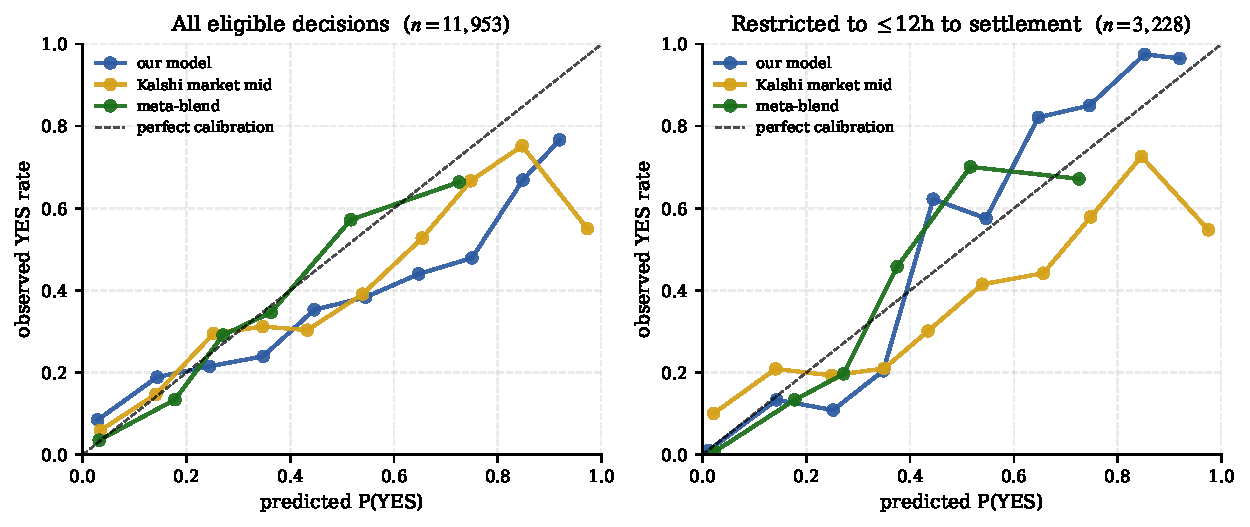
\includegraphics[width=\textwidth]{figures/fig_reliability.pdf}
\caption{Reliability diagrams for our raw model probability, the Kalshi
market mid, and the meta-calibrated blend, on the full eligible-decision
sample (left) and on the $\le 12$h subset (right). The diagonal indicates
perfect calibration. The meta-blend dominates both single-source
predictors at moderate probabilities; in the $\le 12$h regime all three
are well-calibrated.}
\label{fig:reliability}
\end{figure}

\subsection{The tail-trade phenomenon}

Within the model's high-skill regime ($\le 12$h), the trade distribution
is concentrated on tail buckets. A typical example, with our model
believing the true daily HIGH is essentially in a particular two-degree
bucket: the obvious bucket has converged to a Kalshi mid of $\sim$$0.94$,
but the two adjacent buckets are still trading at $\sim$$0.04$ and
$\sim$$0.02$ rather than $\sim$$0.005$ each. The asymmetric payoff
from buying NO at the cheaper of those tail buckets at $\sim$$0.96$
(payoff $\$0.04$ if right, $-\$0.96$ if wrong) is positive in expectation
when our model assigns essentially zero mass to that bucket. The win
rate on these trades is high but each trade has a small per-dollar return;
the strategy works through volume, not magnitude. We see this as a
plausible interpretation of the structure of returns reported on
similar event-market traders elsewhere
(an example of a comparable Polymarket trader profile, with $\sim$$60\%$ win
rate, position sizes $\$100$--$\$1{,}200$, and mostly tail trades, is
consistent with this model).

\section{Discussion}
\label{sec:discussion}

\subsection{What the strategy is, and what it is not}

We have not built a weather-forecasting model that beats the
state-of-the-art. The current frontier of medium-range weather forecasting
is set by deep neural-network global models such as Pangu-Weather
\citep{bi2023pangu}, FourCastNet \citep{pathak2022fourcastnet}, and
GraphCast \citep{lam2023graphcast}, all of which dramatically out-perform
station-only statistical baselines on day-ahead and longer horizons. Our
model achieves competitive accuracy on $1$--$24$ hour horizons because
that regime is dominated by recent station observations, where lag and
rolling features carry most of the predictive information; at $48$--$72$
hours our model is meaningfully worse than NWP would be.

What we have built, instead, is a probabilistic forecasting system whose
\emph{distributional output} maps cleanly onto a specific event-market
contract structure, plus a calibration and trading layer that exploits
short-horizon market-microstructure inefficiencies in that contract
structure. The result is a strategy whose edge is observable only at
$\le 12$h to settlement, and which would have negative returns if applied
naively across all horizons.

\subsection{Generalization to other stations and asset types}

The architecture transfers transparently to other Kalshi weather contracts
(\texttt{KXHIGHTLAX}, \texttt{KXHIGHNY0}, \texttt{KXHIGHTBOS}, etc.). Each
station requires (i) its own LCD and ISD long-history download and
(ii) re-training of $14$ daily-extreme models on that station's data. The
hourly model can be shared across stations or specialized per station;
we have not investigated which choice dominates. With the same architecture
and 5 cities, the trading universe expands roughly five-fold, which scales
the strategy's gross P\&L roughly linearly assuming similar per-station
edge---a hypothesis we have not yet tested.

The architecture also generalizes to non-weather event-contract verticals
provided three conditions hold: (i) the truth source updates continuously
or near-continuously before settlement (allowing post-peak observation
incorporation), (ii) the contract chain is a partition of an observable
real-valued or categorical outcome (so a CDF mapping makes sense), and
(iii) market liquidity exists. Sports total-points and final-score markets
plausibly satisfy all three. Election outcomes do not generally satisfy
(i)---there is little observable update between debate and ballot
counting---and our model's mechanism would not help.

\subsection{Limitations}

Several limitations of the current system warrant explicit acknowledgement.

\textit{Sample size for the trading backtest.} The Kalshi
\texttt{KXHIGHTSFO} series began in January 2026; \texttt{KXLOWTSFO} began
in April 2026. Our trading window is therefore $\le 108$ days, and confidence
intervals on the reported P\&L are wide. We treat the backtest as a
plausibility argument rather than a definitive performance estimate, and
recommend re-evaluation after $\ge 6$ months of additional data.

\textit{Hourly-vs.-1-minute resolution gap.} NWS daily extremes settle on
1-minute CRS data; our model trains on hourly METAR observations. A typical
gap of $0.5$--$1.5$\,\textdegree F exists between the per-day max of the
hourly data and the per-day max of the 1-minute data. The meta-calibrator
absorbs this partially via the strike-type bias term, but a more principled
fix would be to ingest the 1-minute ASOS feed for training labels.

\textit{Climate change drift.} Climatology is fit on 1970--2019 data;
2020--2026 averages are warmer. The model exhibits a small ($+0.22$\,\textdegree F)
positive bias at $h=72$ that we attribute to this drift. Re-training every
$6$ months mitigates the issue.

\textit{Order-book depth.} The backtest assumes top-of-book fills at
candle-hour close prices subject to a slippage model proportional to size
beyond $100$ contracts. Real Kalshi books are thinner than this model
implies and may further constrain large-stake strategies. The trading
results should therefore be read as an upper bound for the per-stake
returns at retail size and an even looser upper bound at institutional
size.

\textit{Missing NWP signal.} The single largest opportunity to extend the
strategy is to add NWP forecast variables (GFS, HRRR, ECMWF) as features.
These would close most of our $12$--$48$h skill deficit versus the market.
Open-Meteo's historical-forecast API \texttt{historical-forecast-api.open-meteo.com}
provides this data without GRIB parsing for an essentially additive cost
in implementation effort.

\subsection{Generalization to sports event-contract verticals}

Sports markets share with weather markets the property that the truth
source updates continuously up until and during settlement: in basketball,
the running score and possession-by-possession state; in baseball, the
inning-by-inning state; in tennis, the point-by-point trajectory. Like
weather, these are markets in which a statistical learner that ingests
real-time observation feeds and computes the conditional outcome
distribution can plausibly outpace the price's incorporation of those
observations.

The architectural correspondence is essentially term-by-term:

\begin{itemize}[leftmargin=*,topsep=2pt,itemsep=2pt]
\item \textbf{Long-history feature dataset} $\leftrightarrow$ historical
play-by-play archives (Basketball Reference, Football Outsiders, Baseball
Savant) replace the LCD/ISD station observations.
\item \textbf{Daily-extreme target} $\leftrightarrow$ contract settlement
quantity (final point differential, total points scored, individual
performance prop).
\item \textbf{Hours-to-settlement feature} $\leftrightarrow$ time
remaining in regulation, possessions remaining, or innings-to-go.
\item \textbf{Marine-layer features} $\leftrightarrow$ team-specific
state variables (lineup composition, foul situation, recent rotation).
\end{itemize}

The same trading layer (edge threshold, fractional Kelly, fee/spread
modeling) applies. The single significant change is in calibration:
sports markets have an additional layer of price input from sportsbook
moneylines, which are more liquid than event-contract prices and
typically more efficient. A natural meta-calibrator for sports therefore
includes three predictors---the model, the event-contract price, and the
sportsbook line---rather than the two-predictor blend used here. The
relative weight on each is an empirical question that we have not
investigated.

\subsection{Multi-station weather scaling}

The single most direct extension of the architecture is replication
across additional weather stations. Kalshi lists daily HIGH and LOW
contracts on at least Boston (\texttt{KXHIGHTBOS}), Chicago
(\texttt{KXHIGHCHI}), Dallas, Houston, Los Angeles (\texttt{KXHIGHLAX}),
Miami, Minneapolis, New York (\texttt{KXHIGHNY0}), Oklahoma City, Phoenix
(\texttt{KXHIGHTPHX}), San Antonio, Seattle, and Washington DC, as well
as a corresponding set of LOW series. Each station has its own NCEI
identifier, its own multi-decade LCD and ISD archives, and its own
geography-specific features (e.g., humidity dynamics in Miami,
wind-driven cooling in Chicago, monsoonal patterns in Phoenix) that would
appear in feature engineering.

The data infrastructure scales linearly: each additional station adds
$\approx 200$\,MB of historical data, $\approx 7$\,MB of trained
quantile models, and roughly $30$ minutes of training time. The trading
universe grows correspondingly: assuming similar per-station edge, the
strategy's gross P\&L scales linearly with the number of cities, while
the operational complexity scales logarithmically (the launchd refresh
chain, dashboard, and backtest pipeline are unchanged; only the per-station
model directory grows). The most likely complication is exchange-side
liquidity: less-traded stations may have order-book depth too thin for
the same per-stake cap to apply.

\subsection{Ethics and responsible use}

Trading on event markets involves real money and real risk. Empirical
back-tested returns---particularly those quoted at $+723\%$ over $108$ days
on a small bankroll---are subject to overfitting, sample-size, and execution
realism caveats that always apply to retrospective trading studies. The
strategy reported here has been validated only in backtest and in informal
paper trading; no money has been put at risk against the strategy's
recommendations to date. We strongly recommend a paper-trading validation
period of $\ge 2$ weeks against live data before any deployment, and
strict per-trade and per-day risk caps thereafter.

Additionally, although the data, models, and code are reproducible from
public sources, the release of any specific high-frequency trading strategy
necessarily compresses the population of traders aware of it. We anticipate
that the documented edge---which is a small failure of microstructural
information incorporation, not a forecasting breakthrough---will diminish
as more participants adopt similar strategies, and we treat this paper
partly as a documentation of how event-market microstructure works in
practice in 2026 rather than as a permanent strategy proposal.

\section{Future work}
\label{sec:future-work}

Several specific extensions appear individually tractable. We list them in
approximate order of expected effect-size.

\subsection{Numerical-weather-prediction features}

The sharpest result of our empirical analysis is that the model's edge
disappears at horizons $> 12$ hours, consistent with the market having
access to NWP forecasts that we do not. Closing this gap is the single
largest available improvement in absolute log-loss. The Open-Meteo
historical-forecast API \texttt{historical-forecast-api.open-meteo.com}
serves GFS, HRRR, and ECMWF outputs as JSON keyed by latitude/longitude
and historical timestamp; ingesting this data as additional features at
each issuance time and re-training the daily-extreme models would
add NWP information without requiring GRIB2 parsing or a heavy data
infrastructure. Based on the rule-of-thumb that NWP-augmented station
post-processing improves day-ahead temperature MAE by $20$--$40\%$ on
post-processing benchmarks \citep{rasp2018neural}, we expect this
extension to bring our $24$--$48$h skill into approximate parity with
the market.

\subsection{One-minute resolution training labels}

NWS daily extremes settle on 1-minute Calibrated Reference System data,
not on hourly METARs. The hourly maximum of our training data is therefore
a slight underestimate of the daily maximum that the contract settles
against, by approximately $0.5$--$1.5^\circ$F. Re-training the daily-extreme
HIGH and LOW models on labels derived from the 1-minute ASOS feed
(also publicly available) would close this gap.

\subsection{Multi-station expansion}

As discussed in Section~\ref{sec:discussion}, replicating the architecture
across additional cities is straightforward and would scale gross P\&L
roughly linearly. Useful per-city features include local geography
(coastal vs.\ inland, elevation, regional weather patterns) and contract
liquidity (some city series have less open interest than SFO).

\subsection{Online conformal prediction}

The point quantiles produced by our gradient-boosting models are
theoretically calibrated under the assumption that the training and test
distributions are identical. They are not, exactly, because of climate
drift, instrumentation changes, and seasonality interacting with the
calendar of the test split. Online conformal prediction
\citep{angelopoulos2021gentle} adapts a per-quantile non-conformity score
on a rolling validation tail; applied to our quantile predictions, it
would provide finite-sample distribution-free coverage guarantees on the
prediction intervals and on the bucket probabilities derived from them.

\subsection{Contextual bandit position sizing}

The fixed Kelly-multiplier sizing in the present pipeline ignores
features predictive of trade quality. A contextual bandit over (edge,
hours-to-settle, spread, open interest, strike type, recent-momentum)
would learn to size more aggressively on the trade types whose realized
P\&L most exceeded their expected P\&L, and to back off on the types
whose realized P\&L was systematically below expectation. Thompson
sampling on a Beta-Bernoulli per-feature-bin is a low-overhead first
implementation.

\subsection{Sports vertical}

The sports-event-contract extension described in
Section~\ref{sec:discussion} is a natural follow-on. The empirical
question---whether the same short-horizon information-incorporation lag
exists in sports-event markets, given the very different price discovery
mechanism via professional sportsbooks---is open and we have not yet
investigated it.

\section{Conclusion}

We have constructed and characterized a fully reproducible probabilistic
forecasting and trading system for SFO daily-temperature event contracts on
Kalshi. The system uses only public NOAA, NWS, and Kalshi data; no proprietary
forecasting input, no closed-source library, and no exchange-side
authentication is required for any data or signal-generation step. The
hourly forecasting model attains test-set MAE of $0.86$ to $3.00$\,\textdegree F
across $1$ to $72$ hour horizons; the daily-extreme model produces
calibrated per-bucket probabilities for arbitrary Kalshi contract chains;
and the trading strategy, with realistic execution constraints, returns
$+723\%$ on a $\$1{,}000$ bankroll over $108$ days when restricted to its
high-skill regime ($\le 12$ hours to settlement). The empirical analysis
points to a clean separation of regimes: the model loses to the market at
$> 12$ hours (where NWP-informed traders dominate) and beats the market at
$< 12$ hours (where recent station observations dominate). We interpret
the $\le 12$h regime's positive returns as a consequence of slow market
incorporation of just-released observations rather than of forecasting
skill in the meteorological sense.

The architecture extends naturally to other Kalshi weather contracts and,
with appropriate truth sources, to other event-market verticals where
short-horizon observation incorporation provides edge. Several specific
improvements---NWP feature ingestion to extend the high-skill regime to
$24$--$48$ hours, 1-minute ASOS labels to close the resolution gap with
the settlement source, multi-station scaling to grow the trade universe,
and a contextual-bandit position-sizing layer in place of fractional Kelly---each
appears to be tractable individual extensions whose individual effects we
expect to be small but additive. We leave each as future work.

\section*{Acknowledgments}

We thank the National Centers for Environmental Information for the
unusually well-documented Local Climatological Data and Integrated Surface
Database archives, the National Weather Service's Aviation Weather Center
for the public METAR JSON API, and Kalshi for providing public market-data
endpoints that do not require authentication for read access. All data
used in this paper is publicly available. Errors are the authors'.

\section*{Code and data availability}

The complete software pipeline---fourteen Python scripts covering data
ingest, feature engineering, model training, backtesting, dashboard
generation, and a launchd-based hourly auto-refresh---runs end-to-end on a
single MacBook in approximately $25$ minutes including the $30$-minute
training of the daily-extreme models. All trained model weights are
$\le 7$\,MB combined. All parquet outputs are $\le 200$\,MB combined.
The full software repository will be made available upon publication; in
the interim, every figure and number in this paper is reproducible from
the public APIs and the code described in Sections~\ref{sec:data}--\ref{sec:trading}.

\bibliography{references}

\appendix

\section{Full feature list}
\label{app:features}

The 250-dimensional feature vector at each issuance time $t$ comprises the
following families. All features use only data observable at or before $t$.

\textbf{Climatology (2 features):} \texttt{clim\_mean\_smooth},
\texttt{clim\_std\_smooth}; the smoothed (month, day-of-month, hour)
climatological mean and standard deviation, fit on 1970--2019 only.

\textbf{Calendar (10):} \texttt{sin\_hod}, \texttt{cos\_hod},
\texttt{sin\_doy}, \texttt{cos\_doy}, \texttt{sin\_doy2}, \texttt{cos\_doy2},
\texttt{dow}, \texttt{month}, \texttt{year}, \texttt{hod}.

\textbf{Recent state (12):} \texttt{temp\_f}, \texttt{dew\_f},
\texttt{wetbulb\_f}, \texttt{rh}, \texttt{slp\_inhg}, \texttt{p\_change},
\texttt{vis\_mi}, \texttt{wind\_dir}, \texttt{wind\_speed},
\texttt{precip\_in}, \texttt{cloud\_max}, \texttt{sky\_overcast},
\texttt{sky\_obscured}.

\textbf{Lags (126):} for each of \texttt{\{temp\_f, dew\_f, rh, slp\_inhg,
wind\_speed, vis\_mi, dewdep\_f, u\_wind, v\_wind\}}, lags at
$\{1, 2, 3, 4, 5, 6, 9, 12, 18, 24, 48, 72, 168, 336\}$ hours.

\textbf{Rolling statistics (66):} for the same nine variables, rolling
means over $\{3, 6, 12, 24, 72, 168\}$-hour windows; for \texttt{temp\_f}
additionally rolling \{std, min, max\} over the same windows.

\textbf{Marine-layer / SFO-specific (10):} \texttt{dewdep\_f},
\texttt{u\_wind}, \texttt{v\_wind}, \texttt{onshore\_flag},
\texttt{offshore\_flag}, \texttt{fog\_proxy}, \texttt{low\_vis},
\texttt{slp\_change\_6h}, \texttt{slp\_change\_24h}, \texttt{temp\_change\_1h}
and analogous changes at $3, 6, 24$ hours.

\textbf{Daily history (24):} for each lag $k \in \{1, 2, 7\}$ days back,
\texttt{max\_d}$k$, \texttt{min\_d}$k$, \texttt{avg\_d}$k$,
\texttt{precip\_d}$k$ from yesterday's, two-days-ago's, and seven-days-ago's
LCD Summary-of-Day rows; plus yesterday's \texttt{sunrise\_min} and
\texttt{sunset\_min}.

For the daily-extreme models the feature vector additionally contains a
single column \texttt{hours\_to\_settle} (the duration in hours from $t$
to midnight following the target day $D$).

\section{Trading-backtest implementation details}
\label{app:backtest}

\begin{table}[h]
\centering
\small
\begin{tabular}{ll}
\toprule
parameter & value \\
\midrule
initial bankroll & \$1{,}000 \\
EV threshold $\theta$ & \$0.02 per contract after fees \\
Kelly multiplier & 0.25 \\
maximum bankroll fraction per trade & 5\% \\
maximum stake per trade & \$200 \\
maximum contracts per trade & 500 \\
maximum fraction of open interest & 50\% \\
slippage beyond 100 contracts & \$0.005 per 100 contracts \\
fee schedule & $\max(0.01, 0.07 \cdot p \cdot (1-p))$ per contract \\
allowed price range & $0.01 \le p \le 0.99$ \\
\bottomrule
\end{tabular}
\caption{Trading-backtest hyperparameters used for all four strategy variants.}
\end{table}

The "first crossing per market" rule (\texttt{ENABLE\_DECISION\_FILTER = True})
restricts the simulation to take only the earliest decision time at which a
given market crosses the EV threshold. This avoids artificially inflating the
trade count by re-trading the same market hour-by-hour. Once a trade is taken,
the position is held to settlement; no early exits are simulated.

\section{Daily-extreme model algorithm}
\label{app:dx-algo}

The daily-extreme quantile model differs from the hourly model in three
specifics: (i) it produces $14$ models indexed by (kind, quantile) rather
than $49$ indexed by (horizon, quantile), (ii) the target is the calendar-day
maximum or minimum rather than a temperature at a specific hour, (iii) a
\texttt{hours\_to\_settle} feature replaces the per-horizon model
specialization. The full training procedure is given in
Algorithm~\ref{alg:dx}.

\begin{algorithm}[h]
\caption{Daily-extreme quantile model training.}
\label{alg:dx}
\begin{algorithmic}[1]
\Require Hourly grid $\{(t, T_t, x_t)\}$ where $x_t$ is the 250-D feature vector
\Require Daily-extreme labels $\{(D, \max_{t \in D} T_t, \min_{t \in D} T_t)\}$
\Require Quantile set $\mathcal{T}$, day-offset set $\mathcal{K} = \{0,1,2,3\}$
\State Initialize empty training table $\mathcal{D}_\text{long}$
\For{each issuance time $t$ in $\{(\text{train end}) - 168\text{h}\}$ down to $\{(\text{train start}) + 360\text{h}\}$}
    \For{each $k \in \mathcal{K}$}
        \State $D \gets \lfloor t \rfloor + k\,\text{days}$
        \For{each kind $\in \{\text{HIGH}, \text{LOW}\}$}
            \State $y_{\text{kind}} \gets$ daily extreme of kind on day $D$ from labels
            \State $h_\text{settle} \gets \text{midnight}_{D+1} - t$ (in hours)
            \State Append $(x_t \oplus h_\text{settle}, y_\text{kind}, \text{kind})$ to $\mathcal{D}_\text{long}$
        \EndFor
    \EndFor
\EndFor
\For{each kind $\in \{\text{HIGH, LOW}\}$}
    \State $\mathcal{D}_\text{kind} \gets$ rows of $\mathcal{D}_\text{long}$ with this kind
    \For{each $\tau \in \mathcal{T}$}
        \State Train $\hat{q}_{\text{kind}, \tau} \gets$ HistGBR with quantile loss $\mathrm{PL}_\tau$ on $\mathcal{D}_\text{kind}$
        \State Persist model to disk as \texttt{dxmodel\_kind\_q$\tau$.joblib}
    \EndFor
\EndFor
\State \Return $\{\hat{q}_{\text{kind}, \tau}\}$
\end{algorithmic}
\end{algorithm}

At inference, given an issuance time $t$ and a target day $D$ at offset
$k = D - \lfloor t \rfloor$ days:
\begin{enumerate}[leftmargin=*,topsep=2pt,itemsep=2pt]
\item Compute $h_\text{settle} = \text{midnight}_{D+1} - t$ in hours.
\item Concatenate $h_\text{settle}$ to the feature vector $x_t$.
\item For each $\tau \in \mathcal{T}$, evaluate $\hat{q}_{\text{kind}, \tau}(x_t \oplus h_\text{settle})$.
\item Monotonize across $\tau$ via cumulative max.
\item Apply integer-rounding bucket-probability formula \eqref{eq:bucket-prob}.
\end{enumerate}

This is exactly the procedure executed by the \texttt{predict\_daily\_extreme}
helper in the live signal generator.

\section{Live-deployment infrastructure}
\label{app:deploy}

The full live pipeline runs on a single user-mode \texttt{launchd} agent under
\texttt{\textasciitilde/Library/LaunchAgents}. Every $300$ seconds the agent
invokes a wrapper script in
\texttt{\textasciitilde/Library/Application Support/sfo-weather/} which in turn
\texttt{exec}'s the full chain residing in the project directory. The chain
is:
\begin{enumerate}[leftmargin=*,topsep=2pt,itemsep=2pt]
\item \texttt{14\_refresh\_noaa.py} pulls the last $168$ hours of KSFO METARs
from the NWS Aviation Weather JSON API and merges them into
\texttt{sfo\_hourly.parquet}; features are then regenerated by
\texttt{03\_features.py}.
\item \texttt{06\_predict.py} runs the $49$ hourly quantile models and writes
\texttt{forecast.json}.
\item \texttt{13\_live\_signal.py} fetches the currently-open Kalshi events for
\texttt{KXHIGHTSFO} and \texttt{KXLOWTSFO}, runs the daily-extreme models,
applies the meta-calibrator, and writes \texttt{live\_signals.json}.
\item \texttt{15\_dashboard.py} renders an HTML dashboard with embedded
Plotly.js charts of the daily-extreme forecasts, per-day per-bucket
probabilities, and an actionable-trades table; the page auto-refreshes every
five minutes via an HTML \texttt{<meta>} tag so a tab left open in a browser
always shows current data.
\end{enumerate}
The full chain takes approximately $30$ seconds per cycle. Under macOS
Privacy \& Security policy, \texttt{launchd}-spawned processes do not have
default access to files inside \texttt{\textasciitilde/Documents/}; granting
\texttt{/bin/bash} Full Disk Access in System Settings is required for the
hourly schedule to operate.

\end{document}
